% Dies ist die Hauptdatei Ihrer Dissertation. Mit * gekennzeichnete
% Elemente sind optional und können durch Entfernen/Hinzufügen des
% %-Zeichens gewählt/abgewählt werden. 


% Dokumentenklasse
%\RequirePackage[patch]{kvoptions} 
%
%\documentclass[inputenc={utf8}]{DissOnlineLatex}
%\usepackage{pdflscape}
%\usepackage[sf,sl,outermarks,compact]{titlesec}
%\makeatletter
%\def\@makechapterhead#1{%
%  {\parindent \z@ \raggedright \normalfont
%    \ifnum \c@secnumdepth >\m@ne
%        \huge\bfseries \@chapapp\space \thechapter
%        \par\nobreak
%        \vskip 20\p@
%    \fi
%    \interlinepenalty\@M
%    \Huge \bfseries #1\par\nobreak
%    \vskip 40\p@
%  }}
%\makeatother

%\newcolumntype{L}[1]{>{\raggedright\let\newline\\\arraybackslash\hspace{0pt}}m{#1}}
\documentclass[pagesize,parskip=full,bibtotoc,12pt]{scrreprt}
% PDF-Kompression
\pdfminorversion=5
\pdfobjcompresslevel=1
% Allgemeines
\usepackage[automark]{scrpage2} % Kopf- und Fußzeilen
\usepackage{amsmath,marvosym} % Mathesachen
\usepackage[T1]{fontenc} % Ligaturen, richtige Umlaute im PDF
\usepackage[utf8]{inputenc}% UTF8-Kodierung für Umlaute usw
\usepackage[official]{eurosym}
\usepackage{url}%für online-Zitate
\usepackage{anysize} %Seitenränder verändern

\usepackage{geometry}
\geometry{a4paper,left=30mm,right=30mm, top=30mm, bottom=30mm}
% Schriften
\usepackage{mathpazo} % Palatino für Mathemodus
%\usepackage{mathpazo,tgpagella} % auch sehr schöne Schriften
\usepackage{setspace} % Zeilenabstand
\onehalfspacing
%\linespread {1.5}\selectfont %Zeilenabstand
%\setlength{\skip\footins}{10mm} 
%\renewcommand{\footnoterule}{%
%  \kern 3pt
%  \hrule width \textwidth height .2pt
%  \kern 2pt
%}
%\newlength{\footnoterulewidth} \setlength{\footnoterulewidth}{1\columnwidth} %\newlength{\footnoteruleheight} \setlength{\footnoteruleheight}{.2pt} \renewcommand{\footnoterule}{
%\kern-3pt \hrule width 5in \kern 6pt
%\kern -3pt \hrule width \footnoterulewidth  \kern 2.6pt
%} 
\renewcommand{\footnoterule}{\vfill\kern -3pt \hrule width 1\columnwidth  height 0.2pt \kern
 10pt}
\usepackage{caption} %Zeilenumbruch in Bildunterschriften

\renewcommand*\chapterheadstartvskip{\vspace*{-1cm}}
\renewcommand*\chapterheadendvskip{\vspace*{5pt}}
% Schriften-Größen

\setkomafont{chapter}{\Large\rmfamily} % Überschrift der Ebene
\setkomafont{section}{\large\rmfamily}
\setkomafont{subsection}{\rmfamily}
\setkomafont{subsubsection}{\rmfamily}

\setkomafont{chapterentry}{\large\rmfamily} % Überschrift der Ebene in Inhaltsverzeichnis
\setkomafont{descriptionlabel}{\bfseries\rmfamily} % für description Umgebungen
\setkomafont{captionlabel}{\bfseries}
%\setkomafont{caption}{\small}
% Nummerierung der Sections und subsections und subsubsections
\setcounter{secnumdepth}{3}

\makeatletter
\renewcommand\section{\@startsection
   {section}{1}{0mm}%      % name, ebene, einzug
   {2\baselineskip}%            % vor-abstand
   {0,1\baselineskip}%            % nach-abstand
   {\bfseries\rmfamily\large}%           % layout
   }
\renewcommand\subsection{\@startsection
   {subsection}{2}{0mm}%      % name, ebene, einzug
   {1\baselineskip}%            % vor-abstand
   {0,05\baselineskip}%            % nach-abstand
   {\bfseries\rmfamily\large}%           % layout
   }
   \renewcommand\subsubsection{\@startsection
   {subsubsection}{3}{0mm}%      % name, ebene, einzug
   {1\baselineskip}%            % vor-abstand
   {0,05\baselineskip}%            % nach-abstand
   {\bfseries\rmfamily}%           % layout
   }
\makeatother 

% Sprache: Deutsch

\usepackage[ngerman]{babel} % Silbentrennung
% PDF
\usepackage[ngerman,hidelinks]{hyperref}
\usepackage[final]{microtype} % mikrotypographische Optimierungen
\usepackage{pdflscape} % einzelne Seiten drehen können
% Tabellen
\usepackage{multirow} % Tabellen-Zellen über mehrere Zeilen
\usepackage{multicol} % mehre Spalten auf eine Seite
\usepackage{tabularx} % Für Tabellen mit vorgegeben Größen
\usepackage{longtable} % Tabellen über mehrere Seiten
\usepackage{array}

\usepackage[table]{xcolor}
%  Bibliographie

% Tabellen

\usepackage{wrapfig}
\addto\captionsngerman{
  \renewcommand{\figurename}{Abb}
} 
% Bilder
\usepackage{graphicx} % Bilder
\usepackage{color} % Farben
\usepackage{colortbl}%Hintergrundfarben für Tabellen	
% Define user colors using the RGB model
\definecolor{dunkelgrau}{rgb}{0.8,0.8,0.8}
\definecolor{hellgrau}{rgb}{0.95,0.95,0.95}
\definecolor{red}{rgb}{1.0,0.5,0.5}
\graphicspath{{images/}}
\DeclareGraphicsExtensions{.pdf,.png,.jpg} % bevorzuge pdf-Dateien
%\usepackage[lflt]{floatflt}
\usepackage{float}
\usepackage{subfigure} % mehrere Abbildungen nebeneinander/übereinander
\newcommand{\subfigureautorefname}{\figurename} % um \autoref auch für subfigures benutzen
\setcapindent{0em} % kein Einrücken der Caption von Figures und Tabellen
%
\setcapwidth[]{0.9\textwidth}
%\setlength{\abovecaptionskip}{0,2cm} % Abstand der zwischen Bild- und Bildunterschrift

%Abkürzungsverzeichnis

\usepackage[]{acronym}


% 
% 
% % Quellcode
\usepackage{listings} % für Formatierung in Quelltexten
\definecolor{grau}{gray}{0.25}
\definecolor{lightgray}{rgb}{.9,.9,.9}
\definecolor{darkgray}{rgb}{.4,.4,.4}
\definecolor{purple}{rgb}{0.65, 0.12, 0.82}



% linksbündige Fußboten
\deffootnote{1.5em}{1em}{\makebox[1.5em][l]{\thefootnotemark}}

%typearea{14} % typearea am Schluss berechnen lassen, damit die Einstellungen oben berücksichtigt werden
% für autoref von Gleichungen in itemize-Umgebungen
\makeatletter
\newcommand{\saved@equation}{}
\let\saved@equation\equation
\def\equation{\@hyper@itemfalse\saved@equation}
\makeatother 
\renewcommand{\labelenumi}{\arabic{enumi}.}
\renewcommand{\labelenumii}{\arabic{enumi}.\arabic{enumii}}

 % Importiere die Einstellungen aus der Präambel
% Eigene Trennungsregeln* 
% FILE: hyphenations.tex  Version 2.1
% AUTHOR:
% Universit�t Duisburg-Essen, Standort Duisburg
% AG Prof. Dr. G�nter T�rner
% Verena Gondek, Andy Braune, Henning Kerstan
% Fachbereich Mathematik
% Lotharstr. 65., 47057 Duisburg
% entstanden im Rahmen des DFG-Projektes DissOnlineTutor
% in Zusammenarbeit mit der
% Humboldt-Universitaet zu Berlin
% AG Elektronisches Publizieren
% Joanna Rycko
% und der
% DNB - Deutsche Nationalbibliothek

\hyphenation{Bei-spiel} 

\usepackage{enumitem}

%-zusaetzliche Kommandos*
%% FILE: appendixA.tex  Version 2.1
% AUTHOR:
% Universit�t Duisburg-Essen, Standort Duisburg
% AG Prof. Dr. G�nter T�rner
% Verena Gondek, Andy Braune, Henning Kerstan
% Fachbereich Mathematik
% Lotharstr. 65., 47057 Duisburg
% entstanden im Rahmen des DFG-Projektes DissOnlineTutor
% in Zusammenarbeit mit der
% Humboldt-Universitaet zu Berlin
% AG Elektronisches Publizieren
% Joanna Rycko
% und der
% DNB - Deutsche Nationalbibliothek

% Eigene Befehle k�nnen hier definiert werden

% Dokumentenanfang
\begin{document}

% Seitennummerierung für Titel, Widmung, Danksagung, Zusammenfassung,
% Inhaltsverzeichnis werden in römischen Zahlen gesetzt
\pagenumbering{roman}
\pagestyle{empty} 

% Titelblatt
%% FILE: titlepage.tex  Version 3.0
% AUTHOR:
% Universit�t Duisburg-Essen, Standort Duisburg
% AG Prof. Dr. G�nter T�rner
% Verena Gondek, Andy Braune, Henning Kerstan
% Fachbereich Mathematik
% Lotharstr. 65., 47057 Duisburg
% entstanden im Rahmen des DfG-Projektes DissOnlineTutor
% in Zusammenarbeit mit der
% Humboldt-Universitaet zu Berlin
% AG Elektronisches Publizieren
% Joanna Rycko
% und der
% DNB - Deutsche Nationalbibliothek

%----------Generierung der Titelseite------------------------------------------

\makeatletter % Diese Zeile darf nicht gesl�scht werden!

\title{ \vspace{-3.5cm}\Huge \@Titel \\ 
\vspace{2cm}
\large{\@Untertitel} \\ 
\vspace{1cm}
%\large{DISSERTATION}}\\ 
%\vspace{1cm}
{\large{Dem \@Fakultaet\  der \\ 
\@Universitaet \\
zur Erlangung des akademischen Grades eines \\
\@Grad\\ 
\vspace{1cm}
eingereichte \@Typ 
}}}





\author{
\raggedright{Vorgelegt von \\  \@Anrede\ \@Vorname\ \@Nachname\ }}
\date{
\raggedright{\@Abgabedatum \\
\vspace{1cm}
Erstgutachterin: \@GutachterA \\
Zweitgutachter: \@GutachterB \\
\vspace{1cm}
%Tag der m\"undlichen Pr\"ufung: \@Pruefungsdatum 
}
}

\makeatother % Diese Zeile darf nicht gel�scht werden!
%\maketitle

% Titelseite
%\clearscrheadings\clearscrplain
\newpage

\begin{center}
\begin{Large}

\vspace{8cm}

\bf Verwaltungsmodernisierung im Westlichen Balkan im Kontext der EU-Erweiterung\\

\vspace{10mm}

 \bf Eine vergleichende Untersuchung am Beispiel von Albanien, Mazedonien und Montenegro\\
\end{Large}
\end{center}
\vspace{8cm}
\begin{large}
\begin{tabular}{p{24cm}}
Dissertation zur \\
Erlangung des akademischen Grades einer \\
Doktorin der Wirtschafts- und Sozialwissenschaften (Dr. rer. pol.) \\
im Fachbereich Wirtschaftswissenschaften\\
der Universität Kassel\\
\end{tabular}

\vspace{3cm}

\begin{tabular}{p{24cm}}
Vorgelegt von Claudia Vollmer\\
Kassel, im Oktober 2013\\
\end{tabular}

\vspace{1cm}

\begin{tabular}{ll}
{\bf Erstgutachterin:} &  Prof. Dr. Silke Laskowski\\
{\bf Zweitgutachter:}&Prof. Dr. Jürgen Reese\\
\end{tabular}
\end{large}
\clearpage

% Widmung*
%% FILE: dedication.tex  Version 2.1
% AUTHOR:
% Universit�t Duisburg-Essen, Standort Duisburg
% AG Prof. Dr. G�nter T�rner
% Verena Gondek, Andy Braune, Henning Kerstan
% Fachbereich Mathematik
% Lotharstr. 65., 47057 Duisburg
% entstanden im Rahmen des DFG-Projektes DissOnlineTutor
% in Zusammenarbeit mit der
% Humboldt-Universitaet zu Berlin
% AG Elektronisches Publizieren
% Joanna Rycko
% und der
% DNB - Deutsche Nationalbibliothek

\thispagestyle{empty}
\vspace*{\fill}
\begin{center}
Dieser Widmungstext ist beispielhaft mittig zentriert. W�nschen Sie
dies nicht, entfernen Sie die beiden \verb \vspace*{\fill} \ oder
\verb \begin{center} \ und \verb \end{center} .
\end{center}
\vspace*{\fill}


% Danksagung*
%% FILE: acknowledgement.tex  Version 2.1
% AUTHOR:
% Universit�t Duisburg-Essen, Standort Duisburg
% AG Prof. Dr. G�nter T�rner
% Verena Gondek, Andy Braune, Henning Kerstan
% Fachbereich Mathematik
% Lotharstr. 65., 47057 Duisburg
% entstanden im Rahmen des DFG-Projektes DissOnlineTutor
% in Zusammenarbeit mit der
% Humboldt-Universitaet zu Berlin
% AG Elektronisches Publizieren
% Joanna Rycko
% und der
% DNB - Deutsche Nationalbibliothek

Danksagungen

% Zusammenfassung/Abstract
%% FILE: abstract.tex  Version 2.1
% AUTHOR:
% Universit�t Duisburg-Essen, Standort Duisburg
% AG Prof. Dr. G�nter T�rner
% Verena Gondek, Andy Braune, Henning Kerstan
% Fachbereich Mathematik
% Lotharstr. 65., 47057 Duisburg
% entstanden im Rahmen des DFG-Projektes DissOnlineTutor
% in Zusammenarbeit mit der
% Humboldt-Universitaet zu Berlin
% AG Elektronisches Publizieren
% Joanna Rycko
% und der
% DNB - Deutsche Nationalbibliothek

%-englische-Zusammenfassung---------------------------------------
\selectlanguage{english}
\begin{abstract}
Here is the english abstract. 				
\end{abstract}

%-deutsche Zusammenfassung----------------------------------------
\selectlanguage{ngerman}
\begin{abstract}
Hier ist Ihre deutsche Zusammenfassung. 
\end{abstract}

  
% Inhalts-, Abbildungs*-, Tabellen*-Verzeichnis
\setcounter{page}{1}
\tableofcontents
\newpage
\listoffigures
\newpage
\listoftables
\newpage

{Verzeichnis der Abkürzungen}

\begin{acronym}
 \acro{KDE}{K Desktop Environment}
 \acro{SQL}{Structured Query Language}
 \acro{Bash}{Bourne-again shell}
 \acro{BdKJ }{		Bund der Kommunisten Jugoslawiens}
 \acro{BENF}{ 		Beneficaries}
 \acro{BiH }{		Bosnia and Herzegovina} 
 \acro{CAF	}{	Common Assessment Framework}
 \acro{CARDS}{ 	European Financing Programme for assisting the countries of the Western Balkans}
 \acro{CCLSGR}{ 	Committee for Coordination of Local Self-Government Reform}
 \acro{CEE 	}{	Central and Eastern European}
 \acro{CEEC 	}{	Central and Eastern European Countries }
 \acro{CoE 	}{	Council of Europe}
 \acro{COMECON}{	Council for Mutual Economic Assistance}
 \acro{CS }{		Civil Service }
 \acro{CSA}{ 		Civil Service Agency (Mazedonien)}
 \acro{DEZA}{	Direktion für Entwicklung und Zusammenarbeit}
 \acro{DG 	}{	Directorate-General}
 \acro{DG ADMIN}{	Directorate-General for Administration}
 \acro{DG ELARG}{	Directorate-General for Enlargement}
 \acro{DG HR	}{Directorate-General for Human Resources}
 \acro{DoPA}{		Department of Public Administration (Albania) }
 \acro{EAR	}{	European Agency for Reconstruction}
 \acro{EAS	}{	European Administrative Space }
 \acro{EBRD}{		European Bank for Reconstruction and Development}
 \acro{EC	}{	European Commission}
 \acro{EGPA}{		European Group of Public Administration }
 \acro{EIPA}{		European Institute of Public Administration }
 \acro{EU	}{	European Union}
 \acro{EuGH}{		Europäischer Gerichtshof}
 \acro{EUPAN}{	European Public Administration Network }
 \acro{FYROM}{	Former Yugoslav Republic of Macedonia }
 \acro{GTZ	}{	Deutsche Gesellschaft für Technische Zusammenarbeit	}
 \acro{HHStA}{	Österreichisches Haus-, Hof- und Staatsarchiv Wien }
 \acro{HRMA}{	Human Resource Management Authority (Montenegro)}
 \acro{IMF	}{	International Monetary Fund}
 \acro{IPA 	}{	Instrument for Pre-accession Assistance}
 \acro{ISPA}{		Instrument for Structural Policies for Pre-Accession}
 \acro{MIFF}{		Multi-Annual Indicative Financial Framework}
 \acro{MIPD}{		Multi-Annual Indicative Planning Document}
 \acro{MPA}{		Master of Public Administration }
 \acro{NGO}{		Non-governmental Organisation }
 \acro{NRO}{		Nichtregierungsorganisation}
 \acro{NISPA}{		Network of Institutions and Schools of Public Administration in Central and Eastern Europe}
 \acro{NPM}{		New Public Management }
 \acro{NUTS}{	Nomenclature des unités territoriales statistiques }
 \acro{OECD}{		Organisation for Economic Cooperation and Development}
 \acro{OSCE}{		Organisation for Security and Cooperation in Europe}
 \acro{OSZE}{		Organisation für Sicherheit und Zusammenarbeit in Europa}
 \acro{PA	}{	Public Administration}
 \acro{PAR	}{	Public Administration Reform}
 \acro{Phare}{		Poland and Hungary Assistance for the Restructuring of the Economy}
 \acro{PIFC}{		Public Internal Financial Control}
 \acro{RESPA}{	Regional School for Public Administration }
 \acro{RGW}{		Rat für gegenseitige Wirtschaftshilfe}
 \acro{SAA	}{	Stabilisation and Association Agreement }
 \acro{SAI	}{	Supreme Audit Institution}
 \acro{SaM}{		Serbia and Montenegro}
 \acro{SAP	}{	Stabilisierungs- und Assoziierungsprozess }
 \acro{SAPARD}{	Special Accession Programme for Agriculture\& Rural Development}
 \acro{SFRJ	}{	Sozialistische Föderative Republik Jugoslawien}
 \acro{SFRY	}{	Socialist Federal Republic of Yugoslavia}
 \acro{SIGMA}{	(OECD) Support for Improvement in Governance and Management}
 \acro{TA	}{	Technical Assistance}
 \end{acronym}


% Seitennummerierung im Hauptteil
\pagenumbering{arabic}
\pagestyle{headings} 

% Kapitel
%\chapter{EU-Beitritt als Option}
Seit dem Ende der kriegerischen Auseinandersetzungen auf dem Balkan in den 1990er Jahren in Folge des Auseinanderbrechens Jugoslawiens besteht für die Länder des Westlichen Balkans \footnote{Kroatien, Serbien, Montenegro und Mazedonien, Albanien, Bosnien-Herzegowina, Kosovo.}  die Option für einen Beitritt zur EU. Allen Staaten des Westlichen Balkans wurde im Juni 2003 vom Europäischen Rat in Thessaloniki eine konkrete EU-Beitrittsperspektive eröffnet. Mazedonien\footnote{Aufgrund eines Namensstreites mit Griechenland ist der offizielle Name „Former Yugoslav Republic of Macedonia“ (FYROM), unter dem das Land 1993 in die Vereinten Nationen aufgenommen wurde. Für einen besseren Lesefluss wird in der vorliegenden Arbeit die Bezeichnung Mazedonien verwendet.}, Montenegro und Serbien haben inzwischen die Stufe von Beitrittskandidaten erreicht, während Albanien, Bosnien-Herzegowina und Kosovo potenzielle Beitrittskandidaten sind. Slowenien, auch ein Nachfolgestaat Jugoslawiens, war schon in der letzten Aufnahmewelle 2004 zusammen mit Ländern Osteuropas in die EU aufgenommen worden, Kroatien ist am 1. Juli 2013 in die EU aufgenommen worden.\par

Der Westbalkan ist von EU-Mitgliedern umgeben (Ungarn, Griechenland, Slowenien, Bulgarien, Italien, Slowakei). So gesehen handelt es sich bei den noch nicht beigetretenen Ländern des Westbalkans quasi um einen „weißen Fleck“ mitten in Europa. Vor dem Hintergrund der fragilen Situation auf dem Balkan nach der Auflösung Jugoslawiens und der potenziell instabilen staatlichen Gebilde (Bosnien-Herzegowina, Kosovo) erscheint eine konkrete EU-Perspektive nachvollziehbar.\par

Für die Europäische Union ist das Bestehen dieses „weißen Fleckes“ ein Problem, für das Lösungen gesucht wurden. Eine anscheinend sinnvolle Lösung ist die erneute Erweiterung der EU mittels der Integration der Länder des Westbalkans. Das Interesse der EU ist dabei auch ein strategisches, nicht zuletzt zur Vermeidung eines Konfliktherdes „vor der Haustüre“. Dieses strategische Interesse schließt gleichzeitig die Hoffnung auf einen Reformmotor mit ein, wie es auch in der folgenden Äußerung Javier Solanas\footnote{Generalsekretär des Rates der Europäischen Union von 1999 bis 2009 und in dieser Zeit Hoher Vertreter für die Gemeinsame Außen- und Sicherheitspolitik (GASP).} zum Ausdruck kommt:\par

„It is in the European interest that countries on our borders are well governed. Neighbours who are engaged in violent conflict, weak states where organised crime flourishes, dysfunctional societies or exploding population growth on its borders all pose problems for Europe. […] The credibility of our foreign policy also depends on the successes achieved in the region. The European perspective is both a strategic goal and an incentive for reform” \cite{solana}.\par

In den Staaten des Westbalkans selbst ist die Aufnahme in die Europäische Union ein vorrangiges Ziel. Damit verbunden sind Hoffnungen auf ein vor allem ökonomisch schnelleres Heranrücken an europäische (Lebens-)Standards.\par

Im Prozess der Ausrichtung der neu entstandenen Westbalkanstaaten auf demokratische Werte und Marktwirtschaft spielten internationale Organisationen seit Anfang der 1990er Jahre eine wesentliche Rolle als Unterstützer sowohl finanzieller Art als auch mit Beratungsleistungen. Im Westbalkan waren dies vor allem das United Nations Development Programm (UNDP), die US-amerikanische Entwicklungshilfeorganisation USAID, die Organisation für Sicherheit und Zusammenarbeit in Europa (OSZE) und die Weltbank sowie die Einrichtung eines Stabilitätspaktes für den Westbalkan (1999). Die EU mit ihrer Agency for Reconstruction (EAR), die in Kosovo, Serbien, Montenegro und Mazedonien die EU-Hilfe koordinierte, kam Ende 2002 hinzu. Ursprünglich war die Hilfe für die neu entstandenen Staaten des Westbalkans auf strukturelle Hilfen und Entwicklungshilfe ausgelegt. Mit zunehmendem Engagement der EU in der Region und nach dem EU-Gipfel von Thessaloniki von 2003 wurde den Ländern des Westlichen Balkans die konkrete EU-Perspektive eröffnet. In der Folge legte die EU für die Region ein Instrumentarium auf, das gezielte EU-Unterstützung im Vorfeld einer möglichen EU-Mitgliedschaft beinhaltete. Die Staaten des Westbalkans werden von der EU als Beitrittskandidaten oder potenzielle Beitrittskandidaten \footnote{Der Statuswechsel von potenziellem Beitrittskandidaten zum Beitrittskandidaten wird vom Rat der EU auf Grundlage einer Stellungnahme der Europäischen Kommission einstimmig entschieden.} durch Programme der pre-accessioning assistance in erheblichem Maße finanziell unterstützt. Diese Instrumente sollen ihnen die Heranführung an Standards ermöglichen, die Voraussetzung für die Aufnahme in die EU sind. Die Unterstützung bezieht sich im Rahmen des Institutionenaufbaus explizit auch auf die Reform der öffentlichen Verwaltung.
\section{Untersuchungsgegenstand}
Für eine Aufnahme in die EU müssen alle zukünftigen Mitgliedstaaten bestimmte Bedingungen erfüllen. Dabei geht es im Wesentlichen um die Annäherung an europäische Standards im Bereich Wirtschaft, Institutionenaufbau und Rechtsstaatlichkeit. Für die erfolgreiche Umsetzung einer Annäherung an die EU muss der gesamte gemeinsame Besitzstand (Acquis communautaire) übernommen werden. Das heißt, die Länder müssen ca. 100.000 Seiten gemeinschaftliche gesetzliche Normen in ihr nationales Recht übernehmen.
Für einen so umfangreichen Prozess, die Übernahme der Europäischen Gesetzgebung in nationales Recht, ist eine effektive öffentliche Verwaltung notwendig.\par
Dennoch ist die Ausgestaltung der öffentlichen Verwaltung im Rahmen des Annäherungsmechanismus kein vorrangiges Thema im Erweiterungsprozess. In den jährlichen Fortschrittsberichten\footnote{Die Fortschrittsberichte der EU werden von der EU-Kommission jährlich im Spätherbst für jedes der Länder erstellt, die einen Beitrittsantrag zur EU gestellt haben. In diesen Berichten wird aus Sicht der EU der Fortschritt des jeweiligen Landes zu den Themen der Kapitel des Acquis communautaire beschrieben.} der EU wird die öffentliche Verwaltung zwar regelmäßig thematisiert, allerdings nur unter politischen Gesichtspunkten. Als wesentlicher Grund hierfür kann gelten, dass der öffentlichen Verwaltung kein eigenes Kapitel im Acquis communautaire zukommt.\par
Im Rahmen der von der EU konzipierten Heranführungshilfe wird (finanzielle) Förderung bereitgestellt, um die Kandidatenländer für die EU „fit“ zu machen. Im Rahmen dieser Heranführungshilfe ist auch die Förderung einer effektiven öffentlichen Verwaltung der Länder im Blick. Der Umfang der finanziellen Förderung für die öffentliche Verwaltung in den Beitrittskandidaten ist allerdings nicht zu vergleichen mit der Förderung von solchen Themen, die im Acquis klar geregelt sind.\par
Es handelt sich gewissermaßen um eine paradoxe Situation. Einerseits ist die öffentliche Verwaltung essenziell wichtig für die erfolgreiche Heranführung von Beitrittskandidaten, andererseits scheint das Thema nicht im Zentrum des EU-Interesses zu stehen.\par
In der vorliegenden Arbeit wird dieser Zusammenhang in den Blick genommen. Die Entwicklung der öffentlichen Verwaltung in drei ausgewählten Ländern des Westlichen Balkans wird von verschiedenen Perspektiven aus betrachtet. Hauptbezugspunkt ist dabei die EU-Perspektive der Westbalkanstaaten in ihrer Bedeutung für die öffentliche Verwaltung.\par
Die Länder des Westlichen Balkans befinden sich mit der EU quasi in einem Verhandlungsprozess. Den Westbalkanländern wird die Mitgliedschaft in der EU in Aussicht gestellt, sie müssen dafür aber bestimmte Bedingungen erfüllen (Konditionalität). Dies ist ein intensiver, wechselseitiger Prozess der Annäherung seitens der Länder, welche die Mitgliedschaft anstreben und seitens der EU, die deren Bemühungen beobachtet, unterstützt und bewertet. \par
Die vorliegende Arbeit untersucht das Verhältnis zwischen den Ländern des Westlichen Balkans und der EU unter dem Gesichtspunkt der öffentlichen Verwaltung. Wichtig ist in diesem Zusammenhang die Darstellung des Status quo der öffentlichen Verwaltung in den drei Untersuchungsländern. Neben der Entwicklung seit der Demokratisierung wird auch die historische Entwicklung der öffentlichen Verwaltung in diesen drei Ländern näher beleuchtet und gefragt, wieweit frühere Zusammenhänge und Entwicklungen in die Gegenwart hinein wirken.\par
Die Untersuchung erfolgt im Wesentlichen auf zwei Ebenen.
\begin{itemize}
\item Die Theorie und Praxis der EU-Erweiterung mit der öffentlichen Verwaltung als Bezugspunkt.
\item Die vergleichende Perspektive am Beispiel der Verwaltungsentwicklung in drei benachbarten Westbalkanländern.
\end{itemize}
Die Kriterien für demokratische und verantwortungsvolle Regierungsführung haben sich international in den beiden letzten Dekaden verändert. Nicht mehr nur formale Parameter wie freie und faire Wahlen, Gewaltenteilung oder Rechtsstaatlichkeit stehen im Fokus der Betrachtung. Zunehmend wird nach „substantive democracy“ gefragt und damit eher outcome-orientierte Kriterien wie Institutionenentwicklung und die Wirkung von „Good Governance“ herangezogen (vgl. \cite{pridham99}). Die Perspektive der europäischen Integration ist dabei ein bestimmendes Moment, denn stabile Regierungspraxis und funktionsfähige Verwaltungsstrukturen sind Voraussetzungen für den Beitritt zur EU und die Übernahme des gemeinschaftlichen Besitzstandes (vgl. \cite{kemmeu}: 49).
\section{Untersuchungsziel}
Ziel der Untersuchung ist eine verwaltungswissenschaftliche Perspektive auf ein bisher eher politikwissenschaftlich bearbeitetes Thema: Die Erweiterung der EU nach Südosteuropa. Eine dezidiert verwaltungswissenschaftliche Herangehensweise erscheint sinnvoll, angesichts des großen Stellenwertes, den die nationalen öffentlichen Verwaltungen der Beitrittsländer im Zuge des Erweiterungsprozesses haben. Die Umsetzung der EU-Aufnahmebedingungen ist in den Beitrittsländern vor allem von der öffentlichen Verwaltung zu leisten. Dennoch ist dieser Zusammenhang von der Forschung bislang wenig beachtet worden. Die vorliegende Arbeit geht erste Schritte zur Schließung dieser bemerkenswert großen Forschungslücke. Erkenntnisse aus der vorliegenden Arbeit könnten bei der Entwicklung von Grundlagen für weitergehende Forschung hilfreich sein.\par
Die Erfahrungen mit der letzten Welle von Ländern, die in die EU aufgenommen wurden, zeigen, dass Verwaltungsreform in ehemals kommunistischen Ländern nicht auf einer tabula rasa stattfindet; vielmehr wurde in vielen Ländern der letzten Erweiterungswelle an Verwaltungstraditionen angeknüpft, die bereits vor der kommunistischen Zeit bestanden. „Revitalization of common administrative roots was helpful for a smooth integration and normalisation of the post-communist state administrations“. (\cite{lipumb05}: 161) \par
Forschungen zur Transformation der vormals zentralistisch organisierten öffentlichen Verwaltungen der letzten EU-Aufnahmenwelle zeigen, dass hier besondere Problemlagen bei der Modernisierung und damit der „Europäisierung“ auftraten.\par
Unter Rückbezug auf die historische Verwaltungsentwicklung in ausgewählten Ländern des Westbalkans lautet die zentrale Frage der vorliegenden Untersuchung:\par
{\bf Welchen Einfluss hat die EU-Perspektive auf die Verwaltungsmodernisierung in den Ländern des Westlichen Balkans?}

Eine Reihe von weiterführenden Fragen schließt sich an:
\begin{itemize}
\item Sind Erfahrungen hinsichtlich der Entwicklung der öffentlichen Verwaltung in den Ländern der letzten Aufnahmewelle übertragbar auf den Westlichen Balkan?
\item  Liefert die historische Betrachtung der Verwaltungsentwicklung unter Einschluss früherer Regime der kommunistischen oder sozialistischen Zeit, aber auch der zeitlich davor gelagerten Einflüsse der Imperien verwertbare Erkenntnisse für den aktuellen Modernisierungsprozess?
\item Wie fördert die EU die Verwaltungsmodernisierung in den Beitrittsländern?
\item Wie schätzen Experten der EU und Akteure im Westbalkan die Verwaltungsentwicklung im Kontext der EU-Erweiterung ein?
\item Welche Optionen bestehen für die Verwaltungsentwicklung in den Westbalkanstaaten?
\end{itemize}
\section{Begründung der Länderauswahl}
In der vorliegenden Arbeit erfolgt eine Länderanalyse von drei benachbarten Staaten des Westbalkans – Mazedonien und Montenegro (Beitrittskandidaten) und Albanien (potenzieller Beitrittskandidat).\footnote{Bosnien-Herzegowina und Kosovo, beide immer noch mit starken internationalen Komponenten in der Administration, wurden von vorneherein ausgeschlossen.} Montenegro und Mazedonien sind Nachfolgestaaten des ehemaligen Jugoslawien. Albanien war von einem isolationistischen kommunistischen Regime geprägt.
\par
Gemeinsames Kennzeichen der Länder des Westbalkans ist die Existenz von großen nicht wettbewerbsfähigen Bürokratien, unterentwickelten Marktwirtschaften, unzureichenden Ressourcen und unzureichender demokratischer Staatlichkeit (Governance). Ineffektive Verwaltungen, in vielen Bereichen Nicht-Erfüllung öffentlicher Aufgaben und Korruption sind weiter bestehende Kennzeichen der öffentlichen Verwaltung in den Westbalkanstaaten. Vor diesem Hintergrund stellt die Reform der öffentlichen Verwaltung im Hinblick auf einen EU-Beitritt eine immense Herausforderung dar.
Eine Länderanalyse des Reformprozesses in drei benachbarten Auswahlländern (Albanien, Mazedonien und Montenegro) ermöglicht einen Vergleich und ggf. Abgrenzung der Problematiken in den untersuchten Ländern. Bei der länderspezifischen Analyse wird neben dem kommunistischen/sozialistischen Vermächtnis auch auf die zeitlich davor bestehenden Verwaltungstraditionen innerhalb des Osmanischen Reiches bzw. Österreich-Ungarns eingegangen. Diese historische Betrachtung ermöglicht Rückschlüsse auf das historische Vermächtnis der unterschiedlichen Verwaltungstraditionen auf den Status quo.\par
Die historisch-kulturelle Gemengelage in den Ländern des Westlichen Balkans wird im Folgenden prägnant charakterisiert: „The countries are both similar and different. They are similar in that all but Albania have a common heritage of modern history -- through their participation in Yugoslavia from 1918 and then their participation in the Socialist Federal Republic after 1945. This heritage has left many traces in law, institutions and exposure to administrative and economic concepts, as well as the involvement in the tragic wars that marked the end of the SFRY. But they are different because of their pre-1918 history. The boundary between the Ottoman and Austro-Hungarian empires ran through the region. The empires deeply marked the legal and administrative systems. The differences include their cultures and traditions, and they are divided amongst Muslim, Catholic and Orthodox peoples“ (\cite{oecd04}: 5).\par
Die Länder der letzten Beitrittswelle im Rahmen der Osterweiterung 2004 \footnote{Bulgarien und Rumänien wurden 2007 aufgenommen.} waren zum ersten Mal Staaten, die einen Systemwechsel von einem kommunistischen zu einem demokratischen Regime vollzogen hatten. Auch die Länder des Westbalkans erlebten einen Systemwechsel, wobei es sich bei dem Sozialismus Jugoslawiens um ein von der staatlichen Verfasstheit der Sowjetunion zu unterscheidendes System handelt. In Jugoslawien wurde eine spezifische Form des Selbstverwaltungssozialismus, in Abgrenzung zur sowjetischen Staatsorganisation umgesetzt. Für die öffentliche Verwaltung bedeutete diese staatliche Verfasstheit einige Ähnlichkeiten mit der kommunistischen Verwaltung, es sind aber auch entscheidende Unterschiede festzustellen. In Albanien hat sich ebenfalls ein von der sowjetischen Staatsorganisation abgegrenztes kommunistisches Regime herausgebildet, wiederum mit spezifischen Ausprägungen in der öffentlichen Verwaltung. Die drei untersuchten Länder unterscheiden sich insofern von den Ländern der letzten EU-Erweiterungswelle, welche die Verwaltungstradition der Sowjetunion übernommen hatten oder Teil der Sowjetunion waren.\par
Bei der detaillierten Betrachtung der historischen Verwaltungsentwicklung in den drei Untersuchungsländern wird deutlich, dass nicht pauschal von einer Verwaltungstradition des Westbalkans ausgegangen werden kann. Es bestehen Unterschiede in der Verwaltungsentwicklung, die zum Teil auf die unterschiedlichen historischen Einflüsse auf die betreffenden Länder zurückgeführt werden können. \par
Die umfassende historische Betrachtung der drei Untersuchungsländer liefert wertvolle Anhaltspunkte für die Beurteilung der zukünftigen Perspektive der EU-Erweiterung im Westbalkan.

\section{Stand der Forschung}
In der Literatur wurden zunächst die aktuellen theoretischen Ansätze gesichtet, die sich mit der Erweiterung der EU und dem Einfluss der EU auf die beigetretenen oder im Prozess des Beitritts befindlichen Staaten beschäftigen. Es handelt sich dabei im Wesentlichen um Untersuchungen, die als „Europäisierungsforschung“ bezeichnet werden können. Diese Ansätze entwickelten sich vor allem in der Politischen Wissenschaft innerhalb der Transitionsforschung. Die Europäisierungsforschung beschäftigt sich mit den Auswirkungen der Mitgliedschaft in der Europäischen Union auf nationale und internationale Prozesse. Im Zuge der Erweiterung der EU nahm die Europäisierungsforschung auch Prozesse im Umfeld der EU-Erweiterung in den Blick.\par
Studien zur Demokratisierung haben eine lange Tradition, während Studien zur Demokratisierung durch Regimewechsel, dem Gegenstand der Transitionsforschung, neueren Datums sind. In diesem Forschungsfeld nehmen Untersuchungen zu den Nachfolgestaaten der Sowjetunion eine große Rolle ein. Besonderes Merkmal dieser Transformation ist die gleichzeitige Neuausrichtung der Länder von einer zentral geplanten Ökonomie hin zu einer marktorientierten Wirtschaftsordnung (\cite{diaman}: 25). Für diejenigen Nachfolgestaaten der Sowjetunion, die inzwischen in die EU aufgenommen wurden, liegen eine Reihe von Studien der Transitionsforschung vor (\cite{dimit02,linden,grab05,kneuer07}). Für die Länder des Westbalkans, die ebenfalls einen Systemwechsel vollzogen haben, ist die Literaturlage dagegen sehr überschaubar. 
\par
Der Transitionsforschung liegen in der Regel zwei Analysekriterien zugrunde: einerseits kulturelle und andererseits politische. Im ersten Fall wird meist auf langfristige Entwicklungen und historische Bedingtheiten abgestellt, die Menschen einschränken. Im Gegensatz dazu wird im letzteren Ansatz das Element der Wahlmöglichkeit stärker betont und von Handlungsoptionen im Zusammenhang mit individuellen und kollektiven Akteuren ausgegangen. Hensell kritisiert die Transformationsforschung zu Osteuropa in ihrer generellen Reduzierung auf den politischen Strukturwandel. Er sieht die analytische Vernachlässigung des bürokratischen Staates in der Forschung als „blinden Fleck“. Untersuchungen zur Verwaltungspraxis wären wünschenswert, auch angesichts der Tatsache, dass der Staatsapparat, zumindest in Teilen, wechselnde Regime überdauert, seien sie dynastischer, kommunistischer oder demokratischer Art (vgl. \cite{hens09}: 27). Aber auch angesichts der Bedeutung der Verwaltungsstrukturen für die Funktionsfähigkeit demokratischer Regierungen ist erstaunlich, wie wenig dieser Aspekt bisher zum Thema politikwissenschaftlicher oder verwaltungswissenschaftlicher Untersuchungen gemacht wurde.
\par
Bereits Mitte der 1990er Jahre haben Linz und Stepan gefordert, einen systematischen Ansatz zur Staatsentwicklung in die Theorien der Transformation zu integrieren (vgl. \cite{linz} 366ff.). Jedoch nur wenige Arbeiten haben ausdrücklich die bürokratisch-staatliche Dimension der Transformation betrachtet. Ergebnis dieser Studien ist, dass sich die staatliche Verwaltung, im Gegensatz zu den politischen Institutionen in vielen Ländern nach dem Ende des Sozialismus, nur langsam wandelt. „Both communist and pre-communist structures and practices are still very much part of today’s bureaucratic order. Instead the overwhelming tendency has been one of structural conservatism. The ‘Big Bang’ of economic reforms has not extended to the administrative sphere, where change has been incremental, ad hoc, and, in the main, un-strategic” (\cite{dimgoe}: 225). 
\par
Ein funktionierender Justizapparat, Polizeiwesen, regelhafte Besteuerung, Fachbeamtentum, formal-rationale Verfahren, nach Max Weber Kernelemente moderner Staatlichkeit, werden in der Transformationsforschung meist vorausgesetzt (vgl. \cite{hens09}: 28).
\par
Es wird deutlich, dass die Erforschung des Verwaltungsumbaus im Zusammenhang mit dem Regimewechsel ein Schattendasein führt. Ebenso wurde das wichtige Thema der Verwaltungsentwicklung im Kontext der EU-Erweiterung bisher von der Forschung nur am Rande behandelt.
\par
Bei Sichtung der Literatur wurde weiterhin gefragt, inwieweit Untersuchungen zur Verwaltungsmodernisierung in den zuletzt in die EU eingetretenen Ländern Osteuropas, vorliegen. Dies geschah im Hinblick auf möglicherweise übertragbare Erkenntnisse auf die EU-Erweiterung nach Südosteuropa. Zu den Ländern Osteuropas, die 2004 bzw. 2007 der EU beitraten, liegen einige Untersuchungen vor, die sich auch mit der Verwaltungsentwicklung beschäftigen. Zu diesem Thema sind mehrere Studien erschienen, die sich vor allem mit der Ausgestaltung des civil service \footnote{In der vorliegenden Arbeit wird der Begriff „civil service“ verwendet. Diese Vorgehensweise erlaubt einen umfassenderen Bezugsrahmen als die deutschen Begriffe Beamtentum, Staatsdienst und öffentlicher Dienst, die jeweils Teilbereiche des civil service bezeichnen.} beschäftigen.
\par
Da der Vergleich dreier Länder des Westlichen Balkans ein zentrales Element der vorliegenden Arbeit ist, wurde die aktuelle Situation der Verwaltungsentwicklung in diesen drei Untersuchungsländern beschrieben. Die Literaturlage ist im Bereich der westlichen Sprachen überschaubar. Vor allem die SIGMA-Initiative der OECD und die Europäische Union haben Studien verfasst, die für die vorliegende Arbeit ausgewertet wurden. Auch einzelne Think Tanks in den jeweiligen Ländern befassen sich mit dem Thema Verwaltungsmodernisierung. Diese Studien wurden ebenfalls berücksichtigt.
\par
Um die möglichen Nachwirkungen der historischen Verwaltung auf die aktuelle Situation in jedem der drei Länder genauer betrachten zu können, wurde die Literatur zur Geschichte der betreffenden Länder gesichtet. Überraschendes Ergebnis dieser Sichtung ist, dass die Ausgestaltung der öffentlichen Verwaltung kaum Thema historischer Darstellungen ist. Allenfalls am Rande kommen die Ausprägungen und die Auswirkungen der Verwaltung in historischen Darstellungen vor. Für die Zeit der sozialistischen bzw. kommunistischen Verfasstheit waren in der Literatur einige Studien zu finden, die sich mit der Verwaltung beschäftigen. Die jeweils zweijährige österreichisch-ungarische Besatzungszeit im ersten Weltkrieg in Montenegro und Albanien ist über Archivmaterial im Österreichischen Staatsarchiv in Wien zugänglich und wurde von der Autorin im Hinblick auf die Beschreibung der historischen öffentlichen Verwaltung vor Ort ausgewertet. Weiterhin knüpft die vorliegende Arbeit an die Masterarbeit der Autorin an, die im Studiengang Master of Public Administration der Universität Kassel verfasst wurde (vgl. Vollmer 2007). Ergänzend zu dieser Masterarbeit wurde 2009 ein thematisch daran anknüpfender Beitrag in der Schriftenreihe „Moderne Verwaltungsentwicklung“ veröffentlicht (vgl. \cite{vollmer09}).
\par
Insgesamt wurde deutlich, dass die Betrachtung der historischen Verwaltung in den Ländern des Westlichen Balkans ein weitgehend unerforschtes Feld ist. Generell findet sich in der Literatur zur Geschichte der Untersuchungsländer in den meisten Fällen ein starker Fokus auf die politischen Entwicklungen, oft unter Einbezug des Einflusses externer Akteure. Die Verwaltungsentwicklung ist bislang kaum im Fokus der Forschung. Die Darstellung und Analyse des Verwaltungssystems im historischen Kontext in länderspezifischer, aber auch regionaler Perspektive könnte sich als lohnend erweisen für zukünftige Forschung. Die vorliegende Arbeit mit Berücksichtigung der historischen Perspektive in der Verwaltungsentwicklung liefert Ansätze in diese Richtung. Aufgrund der weitgehenden Abwesenheit von Literatur zur historischen Verwaltungsentwicklung in den Untersuchungsländern gleicht die Darstellung dieses Themenbereiches allerdings dem Zusammentragen einzelner „Puzzleteilchen“, die einen Eindruck vermitteln, jedoch kein umfassendes Bild abgeben.
\par
Verwaltungsentwicklung und Verwaltungsmodernisierung in den drei Untersuchungsländern werden aus unterschiedlichen Blickwinkeln betrachtet, um auf diese Weise die Zusammenhänge zwischen historischer Entwicklung, Entwicklung seit der Demokratisierung und der EU"=Perspektive soweit wie möglich auszuleuchten.

\subsection{Verwaltungsreform/Verwaltungsmodernisierung }
Zentral für die vorliegende Untersuchung ist das Konzept von „Governance“, bzw. „Good Governance“, auch „Gute Regierungsführung“. Good Governance kann als Weiterentwicklung der unterschiedlichen nationalen Verwaltungstraditionen im Zuge der zunehmenden Internationalisierung und Globalisierung verstanden werden.
\par
Die spezifische Ausrichtung der Modernisierung der öffentlichen Verwaltung wird im Wesentlichen bestimmt durch den jeweiligen historischen und kulturellen Kontext der Verwaltungsentwicklung. In Europa werden grundsätzlich vier verschiedene Verwaltungstraditionen unterschieden. Unterschieden wird in kontinentaleuropäisch-deutsche Tradition, kontinentaleuropäisch-französische (napoleonische) Tradition, angelsächsische Tradition und skandinavische Tradition als Mischung der angelsächsischen und deutschen Tradition (vgl. \cite{lipumb05}: 61). Hill fragt, ob nicht auch von einer spezifischen südeuropäischen Verwaltungstradition ausgegangen werden muss, und vor allem von einer mittel- und osteuropäischen Verwaltungstradition (vgl. \cite{hill06}: 15). Es wird also deutlich, dass es nicht „die” öffentliche Verwaltung gibt, die als Modell dienen kann \footnote{In den Institutionen der Europäischen Union finden sich Elemente aller dieser Traditionen.}.
\par
Die europäischen Verwaltungstraditionen sind im folgenden Schema im Überblick dargestellt:\footnote{Für eine detailliertere Beschreibung der Kennzeichen der vier Modelle von Verwaltungsstilen siehe Anhang }.
\begin{figure}[H]
  \centering
  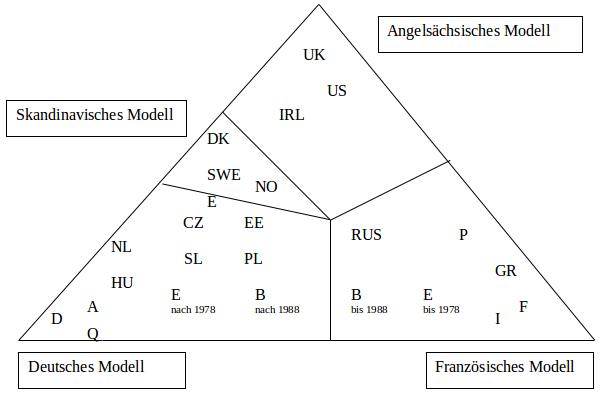
\includegraphics[width=5in]{Material/VerwaltungsModelle}
  \caption{Quelle: Lippert/Umbach 2005 \cite{lipumb05}: 68}
\end{figure}

Aus dem Überblick wird erkennbar, dass es in der EU kein gemeinsames Modell gibt, nach dem eine öffentliche Verwaltung organisiert ist. Vielmehr gibt es nach dieser Darstellung vier Haupttraditionen, die eng mit der historischen Entwicklung in den einzelnen Ländern verbunden sind. Dass die Orientierung in eine bestimmte Richtung nicht statisch ist, zeigen die Beispiele Belgien und England, deren Administrationen zunächst dem französischen Modell angelehnt waren und nun eher dem deutschen Modell folgen, wie im obigen Schema ersichtlich. Weiterhin unterliegen die öffentlichen Verwaltungen Einflüssen, die aus einer generellen Internationalisierung resultieren. So hat das Konzept des „New Public Management“ in allen EU-Mitgliedstaaten zu einem Umdenken und vielfach auch Umbau der Verwaltungen geführt (vgl.\cite{dunhoo}).
\par
Die Modernisierung der öffentlichen Verwaltung ist weltweit in fast allen Ländern zum Thema geworden. In vielen Ländern auf allen Kontinenten sind Aktivitäten zu verzeichnen, deren Ziel eine rationale und effektive Verwaltungsführung ist. Damit verbunden ist meist die Hoffnung auf Kosteneinsparungen, die konsequente Trennung von Verwaltung und Politik, größere Bürgernähe der Verwaltung und/oder verbesserte Aufgabenerfüllung der öffentlichen Hand. Dabei sind mehrere Beweggründe für Verwaltungsmodernisierung zu beobachten:
\par
\begin{itemize}
\item In Ländern mit entwickelten öffentlichen Verwaltungen die Notwendigkeit, Ausgaben im öffentlichen Sektor einzusparen.
\item In Transformationsländern mit nicht existenten Verwaltungsstrukturen oder vormals Kommandowirtschaft die Notwendigkeit, Verwaltungsstrukturen nach modernen Kriterien aufzubauen.
\item Internationale Ausrichtung, z.B. EU-Mitgliedschaft.
\item Globalisierung: Wettbewerb der Länder untereinander bei der Schaffung optimaler Bedingungen für global operierende Unternehmen und Investoren.
\end{itemize}
Man kann zwei Phasen unterscheiden bei dem Austausch von Erfahrungen zwischen Ländern im Feld öffentlicher Verwaltung. Die erste Phase bestand ungefähr von den 1970er Jahren bis Ende des 20. Jahrhunderts. Diese Phase war geprägt von Informalität, Spontaneität und Freiwilligkeit. Kennzeichen war die gegenseitige Beeinflussung der administrativen Systeme, basierend auf Verwaltungsrecht und Gewohnheitsrecht, sowohl in Europa als auch in der Welt. Die zweite Phase des Austausches von Erfahrung und Wissen im Bereich öffentlicher Verwaltung ist seit Beginn des 21. Jahrhunderts auszumachen. Die Überzeugung, dass man die nationalstaatlichen öffentlichen Verwaltungen nicht nur sich selbst überlassen sollte, wurde in der Milleniumserklärung der Vereinten Nationen 2000 in den Blick genommen, die die enge Verzahnung des Kampfes gegen Armut und das Recht auf Entwicklung und „Good Governance“ definierte. 
\subsection{Das Konzept „Good Governance”}
In der vorliegenden Arbeit wird der Begriff „Reform der öffentlichen Verwaltung“ (Englisch: Public Administration Reform, PAR) in einem umfassenden Sinne verstanden; er umfasst den Beamtenapparat, seine rechtliche Verankerung, seine Funktionen, Kompetenzen und Verfahren, unter Einschluss der Verwaltung des Justizsystems. Über den klassischen Begriff der öffentlichen Verwaltung hinaus wird ein umfassenderes Konzept von ‘governance’ zugrunde gelegt. Dieses schließt die Kultur des Regierungshandelns im Sinne der nationalen Entscheidungen hinsichtlich der Ausgestaltung von Staatlichkeit (Legitimität, Effektivität, Transparenz, Pluralität und Verantwortlichkeit) ein, ebenso wie die Beziehungen zwischen Regierung und Parlament.\par
Der Begriff Governance, der zentral ist in der Betrachtung der Verwaltungsmodernisierung in den Ländern, die einen EU-Beitritt anstreben, wird von verschiedenen Institutionen unterschiedlich beschrieben.\par
Die Vereinten Nationen gehen von einer umfassenden Definition von „Governance“ aus, die die Definition einer modernen öffentlichen Verwaltung einschließt. „Governance“ im Gegensatz zum traditionellen Verständnis von „Öffentlicher Verwaltung“ legt einen Schwerpunkt auf Mitgestaltung und Partnerschaft. „Public administration needs to be transformed into a responsive instrument to meet the needs of all citizens“ (\cite{unpan}).\par
Das gewachsene Interesse an einer Governance-Orientierung der Vereinten Nationen wird auf folgende Entwicklungen zurückgeführt:
\begin{itemize}
\item den Erfolg der Marktwirtschaft und das Scheitern der Planwirtschaft;
\item die Tendenz, demokratische Regierungsformen mit wirtschaftlichem Erfolg gleichzusetzen;
\item die weltweite Krise der öffentlichen Finanzen, die in vielen Staaten die Frage nach der Rolle und der Effizienz des Staates neu gestellt hat; 
\item die gestiegene Wahrnehmung und Verärgerung über Korruption in Regierung und Verwaltung;
den Zusammenbruch der ehemaligen Sowjetunion und die ethnischen Konflikte auf dem Balkan und in Afrika, die die neuen Staaten vor große Umbauaufgaben auch ihres politischen Systems stellen (vgl. \cite{undp}: 18).
\end{itemize}
Die Weltbank beschreibt das Konzept als “the traditions and institutions by which authority in a country is exercised for the common good” (\cite{weltbank}: 1). Die sechs Governance-Indikatoren der Weltbank gelten mittlerweile als Standardkriterien zur Bewertung von Good Governance: 
\begin{itemize}
\item Politische Mitspracherechte (Voice and Accountability),
\item Politische Stabilität und Gewaltkontrolle (Political Stability and No Violence);
\item Effektivität des Regierens (Government Effectiveness),
\item Qualität regulativer Politik (Regulatory Quality),
\item Rechtsstaatlichkeit (Rule of Law),
\item Korruptionskontrolle (Control of Corruption) (vgl. \cite{kaufmann}).
\end{itemize}
Im Laufe der 1990er Jahre übernahmen auch die in der OECD zusammengeschlossenen Geber sowie die EU das Konzept der „guten Regierungsführung“.\par
Die SIGMA-Initiative der OECD versucht in ihrer Veröffentlichung zu ‘European Principles of Public Administration’ im Jahr 1999, ebenfalls an den Weltbankindikatoren angelehnt, Prinzipien für die öffentlichen Verwaltungen in ihren Mitgliedstaaten aufzustellen. Folgende Indikatoren werden genannt: 
\begin{itemize}
\item reliability and predictability (legal certainty or judicial security); 
\item openness and transparency; 
\item accountability; 
\item efficiency and effectiveness (vgl. \cite{oecd99}: 8ff).
\end{itemize}
An dem Good-Governance-Verständnis von Weltbank und IWF sowie OECD orientiert sich auch die Europäische Union. Die Europäische Kommission hat im Jahr 2001 ihr Weißbuch „Europäisches Regieren“ veröffentlicht, das ebenfalls Kriterien guter Regierungsführung enthält (vgl. \cite{czada2010}). Dort werden folgende Prinzipien als Merkmale von Good Governance definiert:
\begin{itemize}
\item Transparenz: Institutionen sollten in ihrem Handeln transparent sein und erklären, wie ihre Entscheidungen zustande kommen.
\item Partizipation: Die Qualität und Effektivität von Politik hängt wesentlich von umfassender Partizipation ab.
\item Übernahme von Verantwortung: Institutionen müssen erklären, warum sie etwas tun, und auch dafür Verantwortung übernehmen.
\item Effektivität: Policies müssen effektiv und zeitnah umgesetzt werden mit dem Ziel, das Benötigte auf der Basis von definierten Zielen zu liefern.
\item Kohärenz: Policies und Handlungen müssen kohärent und nachvollziehbar sein.
(vgl. \cite{euko01}: 13).
\end{itemize}
Gute Regierungsführung ist demnach im Wesentlichen gleichbedeutend mit einer leistungsfähigen, berechenbaren und transparenten staatlichen Verwaltung. Sie setzt „ein funktionierendes öffentliches Buchführungs- und Rechnungswesen ebenso voraus wie einen verbindlichen rechtlichen Rahmen, der privatwirtschaftlichen Wettbewerb ermöglicht“ (\cite{schmitz09}: 132).
\par
In der Debatte um die Notwendigkeit stabiler Institutionen und einer effektiven öffentlichen Verwaltung schwingt explizit oder implizit mit, dass die Modernisierung der öffentlichen Verwaltung die Demokratisierung vorantreibt. „Die Demokratie ist heute eigentlich keine Volksregierung, sondern eine Volksverwaltung – die Administration ist die eigentliche Aufgabe der Demokratie“ (Masaryk, zit. nach \cite{czerwick}: 14). Czerwick merkt dazu an, dass in der wissenschaftlichen Literatur davon ausgegangen wird, dass demokratische Systeme nur überleben können, wenn sichergestellt ist, dass die öffentlichen Verwaltungen ein Mindestmaß an struktureller Übereinstimmung mit demokratischen Normen, Institutionen und Prinzipien aufweisen.
\par
Vor diesem Hintergrund ist im Zusammenhang mit der (weiteren) Demokratisierung der Staaten des Westlichen Balkans und ihrem Wunsch einer Aufnahme in die Europäische Gemeinschaft die Frage nach dem Status quo der Verwaltung in diesen Ländern unumgänglich. Es wird deutlich, dass die öffentliche Verwaltung ein zentrales Element ist für die weitere Entwicklung, Demokratisierung und ultimativ den EU-Beitritt der Balkanstaaten. Dennoch ist dieser Zusammenhang von der Forschung bislang wenig beachtet worden. Die vorliegende Arbeit versucht erste Schritte, um diese bemerkenswert große Forschungslücke zu schließen. In Anbetracht der kaum vorhandenen Literatur wird das Thema Verwaltungsmodernisierung im Westbalkan im Kontext der EU-Erweiterung in der vorliegenden Arbeit von mehreren Seiten betrachtet. Die historische Perspektive fließt mit ein, in der Hoffnung auch aus dieser Betrachtung Hinweise zur Beantwortung der Forschungsfragen zu erhalten.
\section{Methodisches Konzept}
In der vorliegenden Arbeit wird eine Annäherung an ein bisher weitgehend nicht untersuchtes Thema, die Bedeutung der Reform der öffentlichen Verwaltung im Westlichen Balkan im Kontext der EU-Erweiterung, vorgenommen. Da mit dieser Untersuchung quasi Neuland betreten wird, wurde eine Methode gewählt, die es ermöglicht, das Thema von unterschiedlichen Seiten aus zu betrachten. Gewählt wurde ein kaleidoskopisches Verfahren, mittels dessen versucht wird, Antworten auf die zentrale Frage und die weiterführenden Fragen der Untersuchung finden. Die Vorgehensweise in der vorliegenden Arbeit ist im Rahmen des Forschungsansatzes der Triangulation verortet. Triangulation findet vor allem in der empirischen Sozialforschung Anwendung. Mit unterschiedlichen Methoden oder Sichtweisen, bzw. Daten wird versucht ein Phänomen zu erklären. Ursprünglich kommt der Begriff Triangulation aus der Landvermessung, wo er folgendermaßen verwendet wird:\par
„Triangulation is the method of location of a point from two others of known distance apart, given the angles of the triangle formed by three points. By repeated application of the principle, if a series of points form the apices of a chain or network of connected triangles of which the angles are measured, the lengths of all the unknown sides and the relative positions of the points may be computed when the length of one of the sides is known” (\cite{clark}: 145).\par
In der sozialwissenschaftlichen Forschung wurde die Triangulation als Methode entwickelt, um von verschiedenen Referenzpunkten aus die Position des (Forschungs-)Objektes zu lokalisieren (vgl. Smith 1975, zit. nach \cite{jick}: 136). Auf dieser Grundlage definiert Flick: „Triangulation beinhaltet die Einnahme verschiedener Perspektiven auf einen untersuchten Gegenstand oder allgemeiner: bei der Beantwortung von Forschungsfragen. Diese Perspektiven können sich in unterschiedlichen Methoden, die angewendet werden, und/oder unterschiedlichen gewählten theoretischen Zugängen konkretisieren, wobei beides wiederum miteinander in Zusammenhang steht bzw. verknüpft werden sollte. Weiterhin bezieht sie sich auf die Kombination unterschiedlicher Datensorten jeweils vor dem Hintergrund der auf die Daten jeweils eingenommenen theoretischen Perspektiven“ (\cite{flick08}:12).\par

In ähnlicher Weise resümiert Schirmer: „Triangulation meint – allgemein gesprochen – die Betrachtung eines ‚Punktes’ aus mehreren Perspektiven mit dem Ziel, diesen Punkt umfassender oder vollständiger zu verstehen, sozusagen ein kompletteres Bild zu entwerfen; damit sollen gleichzeitig Verzerrungen oder Fehlblicke vermieden oder relativiert werden, die Resultat einer bestimmten Perspektive sind.“ (\cite{schirmer}: 100). \par
Der Kern der Triangulation als Methode in der sozialwissenschaftlichen Forschung ist die Kontrastierung. In der vorliegenden Arbeit werden die Erkenntnisse aus der Literaturanalyse anhand von Interviews mit Experten überprüft und so eine Kontrastierung vollzogen, die möglicherweise zu neuen Erkenntnissen und weiterführenden Fragestellungen führt. Diese Vorgehensweise erscheint als eine gute Grundlage für weitergehende Forschung zu dem bisher wenig beleuchteten Thema dieser Arbeit.\par

In der praktischen Anwendung kann man zwei unterschiedliche Lesarten zu Triangulation feststellen. Im ersten Fall wird die Triangulation als Validierung von Forschungsergebnissen durch die Verwendung unterschiedlicher Methoden gesehen. Eine andere Lesart ist die Triangulation mit dem Ziel, ein umfassenderes Bild des Gegenstandsbereichs zu erzielen und den Untersuchungsgegenstand von unterschiedlichen Perspektiven her zu betrachten (vgl. \cite{kelle}: 50). Für die vorliegende Untersuchung wird die Triangulation im letzteren Sinne verwandt.
\par
Es wird versucht, über eine Betrachtung der historischen Verwaltungstradition und Verwaltungsentwicklung in drei benachbarten Ländern des Westlichen Balkans (Albanien, Mazedonien und Montenegro) Gemeinsamkeiten und Unterschiede aufzuspüren, die für den Status quo der Verwaltungsentwicklung in den Ländern relevant sein könnten.\par
Der aktuelle Bezugspunkt der Untersuchung und allen drei Untersuchungsländern gemein ist die Aufnahmeperspektive in die EU. Neben der Entwicklung der Beziehungen der Untersuchungsländer zur EU wird daher auch die Unterstützung der EU im Rahmen der Heranführungshilfe für die Aufnahmekandidaten beschrieben.\par
In einem weiteren Teil der Arbeit werden von der Verfasserin durchgeführte Experteninterviews zu den Forschungsfragen der Arbeit ausgewertet. Die Interviews betreffen thematisch den Status quo der Verwaltungsmodernisierung in den Untersuchungsländern und die Unterstützung durch die EU. Sechs Interviews wurden hierzu mit hochrangigen Beamten der EU und OECD / SIGMAs durchgeführt. Um die Perspektive in den Untersuchungsländern zu erfassen, wurden außerdem in jedem der drei Länder jeweils ein Vertreter der Regierung und ein Vertreter einer Nichtregierungsorganisation (NRO/NGO) interviewt. Alle Interviewpartner waren intensiv mit Verwaltungsmodernisierung befasst und sind in diesem Sinne Experten zum Thema. Insgesamt wurden also zwölf Interviews durchgeführt, die für die vorliegende Arbeit ausgewertet wurden.
\par
In Anbetracht der noch sehr überschaubaren Literatur zum Prozess der Verwaltungsmodernisierung in den Westbalkanländern unter dem Einfluss des EU-Erweiterungsprozesses stellt die Auswertung der Experteninterviews einen unverzichtbaren Beitrag dar. Dabei geht es nicht vorrangig um die Validierung von Ergebnissen der Literaturdurchsicht, sondern um eine Erweiterung der Forschungsperspektive unter Einschluss der persönlichen Erfahrungen und Meinungen von Experten, die sich mit dem Thema in der täglichen Berufspraxis beschäftigten.\par
In die vorliegende Untersuchung fließen ferner Eindrücke aus der eigenen beruflichen Praxis ein. Die Verfasserin hat mehrere Jahre für die OSZE in Südosteuropa im Bereich Demokratisierung vor allem in der Durchführung und Beobachtung von Wahlen gearbeitet (Kosovo noch unter internationaler Administration, Bosnien-Herzegowina, Albanien und Montenegro). Ein wiederkehrender Befund durchzieht diese jahrelange Beschäftigung. Einerseits handelt es sich bei dieser Region geografisch um Europa. Im gemeinsamen Land Jugoslawien bestanden über viele Jahre politisch und ökonomisch enge Kontakte mit den Ländern der EU und der EU als Institution. Andererseits erscheint die Region heute weit von Europa entfernt. So findet Berichterstattung in den westeuropäischen Medien kaum statt. Dieses mangelnde Interesse kann nur zum Teil mit den Kriegen Anfang der 90er Jahre erklärt werden, die zu ökonomischen und politischen Rückschritten führten.\par
Der Widerspruch zwischen einerseits geografischer Zugehörigkeit zu Europa und andererseits wahrnehmbar großer Entfernung zu Westeuropa spiegelt sich auch in der Herangehensweise der EU gegenüber der Region. Einerseits hat die EU den Staaten des Westbalkans seit 2003 einen Beitritt zur EU in Aussicht gestellt. Andererseits sind Auflagen seitens der EU formuliert worden, die in wesentlichen Punkten über die Anforderungen der früheren Aufnahmewellen hinausgehen. Auch wird die bisher gängige Praxis einer gemeinsamen EU-Aufnahme mehrerer Staaten für die Länder des Westbalkans ausgeschlossen.
\section{Aufbau der Arbeit }
Übergeordneter Bezugsrahmen für die vorliegende Arbeit ist zunächst die Konditionalität der EU, die derzeit den theoretischen Hauptstrang der Europäisierungsforschung darstellt. Das Konzept der Konditionalität wird im zweiten Kapitel aus der Demokratisierungs- und Transformationsforschung hergeleitet und bildet den ersten Rahmen der Untersuchung.
Ebenfalls im zweiten Kapitel wird der Prozess der EU-Erweiterung in der Praxis dargestellt. Dabei wird auch ausführlich auf den Stellenwert der Verwaltungsmodernisierung in diesem Prozess eingegangen. Hierbei ist zentral, dass Verwaltungsentwicklung im Erweiterungsprogramm der EU nicht explizit vorkommt. Eine implizite Bezugnahme ist dennoch erkennbar mit dem Konzept des Europäischen Verwaltungsraums, das ebenfalls dargestellt wird. Für dieses Kapitel werden Veröffentlichungen der EU und anderer internationaler Akteure (OECD/SIGMA, UNDP, Weltbank usw.) hinsichtlich des Stellenwertes von Verwaltungsentwicklung innerhalb des Erweiterungsprozesses ausgewertet. Ein wichtiger Teilaspekt der Betrachtung in diesem Kapitel ist die Auswertung der letzten Aufnahmewelle der EU hinsichtlich der Erfahrungen mit und der Nachhaltigkeit von Verwaltungsmodernisierung. Abschließend werden im zweiten Kapitel die Hilfen der EU für die Verwaltungsentwicklung in Kandidatenländern vorgestellt. \par
Die Ausgangslage auf dem Westbalkan ist Gegenstand des dritten Kapitels und bildet einen weiteren Rahmen für die Arbeit. Es wird auf die sozialistische (Jugoslawien) und kommunistische (Albanien) Verwaltungsgeschichte ebenso eingegangen wie auf die zeitlich davor gelagerten imperialen Einflüsse auf die Verwaltung (Österreich-Ungarn, Osmanisches Reich). Dieser Teil der Arbeit wird vorwiegend mittels einer Literatur-Auswertung durchgeführt. Auch die Sichtung von Akten der Österreichischen Militärverwaltung in Montenegro und Albanien während des Ersten Weltkrieges durch die Autorin im Staatsarchiv in Wien fließt in diesen Teil der Untersuchung ein. Als Bezugsrahmen dieses Teiles der Arbeit dient der Legacy-Ansatz, der auch für die vergleichende Verwaltungsforschung anwendbar ist. An die historische Betrachtung schließt sich die kursorische Darstellung der Verwaltungsentwicklung in den drei Untersuchungsländern in der Demokratie an.
\par
Der empirische Teil der Arbeit folgt im vierten Kapitel, bestehend aus zwölf Experteninterviews. Im ersten Teil dieses Kapitels wird die angewandte Methode für die Durchführung der Experteninterviews dargestellt, einschließlich des Vorgehens bei der Auswertung. Im Hauptteil des vierten Kapitels werden die Ergebnisse der Experteninterviews analog der behandelten Themenstränge dargestellt und analysiert.\par
Das Gesamtergebnis der Untersuchung wird im fünften Kapitel zusammengefasst dargestellt.
\chapter{Forschungsansätze zum politischen Wandel in Europa }
Prozesse des politischen Wandels sind weltweit mit unterschiedlicher Intensität und aufgrund verschiedenartiger Impulse unter dem Einfluss unterschiedlicher Rahmenbedingungen zu beobachten. Schwerpunkte sind die Umwandlung traditionell regierter Länder zu modernen Staaten, wie insbesondere im Rahmen der westlichen Entwicklungshilfe, und aktuell die Umwälzungen in Nordafrika, sowie die Transformation vormals sozialistisch beherrschter Länder in demokratisch regierte Staaten in Osteuropa. Die Aufnahme von Staaten in die Europäische Union stellt für diese ebenfalls einen grundlegenden Wandel dar, zu dessen Beschreibung und Gestaltung allgemeine Forschungsergebnisse aus den verschiedenen Prozessen des politischen Wandels herangezogen werden können. Die Forschungsrichtung der Europäisierungsforschung und hier insbesondere das Konzept der Konditionalität ist der vorherrschende Ansatz zur Erklärung verschiedenster Prozesse, welche die EU als supranationale Organisation entfaltet. Die Europäisierungsforschung wird in diesem Kapitel als zentraler Ansatz ausführlich dargestellt, insbesondere die in ihrem Umfeld entwickelte Konditionalitätsforschung. Diese Forschungsrichtung ist von besonderer Bedeutung für die vorliegende Arbeit, da die Verwaltungsmodernisierung ein wesentliches Element der EU-Bedingungen für die Aufnahme der Westbalkanstaaten ist. Im Folgenden werden diese Forschungsrichtungen aus der Transitionsforschung hergeleitet mit den konkreten Fragestellungen der Europäisierungsforschung und der Konditionalitätsforschung. 
\section{Transitionsforschung}
Die Transitionsforschung, die sich traditionell mit Entwicklungsländern beschäftigte, erfuhr durch die politische Wende in Osteuropa eine neue Ausrichtung. Nach dem Systemwechsel in den Ländern Mittel- und Osteuropas war die wissenschaftliche Aufarbeitung der Geschehnisse zunächst von wirtschaftswissenschaftlichen Konzeptionen beherrscht, die sich vor allem mit dem Wechsel der Wirtschaftsweise von zentraler Planwirtschaft zu Marktwirtschaft befassten. Die auch stattfindenden politischen Transformationsprozesse wurden in der Folge ebenfalls nach und nach mit Erklärungsmodellen begleitet. Es entstanden Staatenanalysen und Untersuchungen spezifischer Systembereiche mit ökonomischem, demokratietheoretischem oder soziologischem Schwerpunkt (\mbox{vgl. \cite{huszak}: 54ff}).\par
König definiert den Prozess der Transition in den neu entstandenen Ländern Osteuropas eher als einen der Transformation. „It is evident that in the transition from command to market economy and from totalitarian state to a pluralist state, creating multiparty democracy is not only a transition in itself but rather a long process of transformation. It requires essential reforms in the basic functions and institutions of the state” (König 1992, zit. nach \cite{jenei}). \par
Der Einfluss der EU als einer der wesentlichen Geber kam zunehmend in den Blick als externer Akteur der Transformation. Von Beyme konstatiert in diesem Zusammenhang, dass der „internationale Einfluss der etablierten Demokratien auf die neuen Systeme (…) eine neue Dimension in der Weltgeschichte“ darstellt (\cite{beyme}: 158). Whitehead geht von drei Formen der Demokratisierung aus, erstens der auferlegten Demokratisierung, zweitens Demokratisierung durch Dekolonisierung und drittens Demokratisierung durch Konvergenz (vgl. \cite{whitehead}). Pridham entwickelt ein Konzept der interaktiven Prozesse zwischen externen (vor allem internationalen Organisationen) und innerstaatlichen Akteuren (vgl. \cite{pridham91,pridham95,pridham08}), während das Konzept der Diffusion bzw. einer Art „Schneeballeffekt“ bei der Demokratisierung von Huntington stammt (vgl. \cite{hunting}). Eine Aufarbeitung des Systemwandels in Osteuropa unter Betrachtung externer Faktoren findet statt; diese werden allerdings noch nicht in einem ausreichenden Maße in theoretische Erklärungszusammenhänge eingebunden: „…even though the influence of international factors has been widely acknowledged, these still have not been fully integrated into theoretical frameworks aiming to explain the dynamics or failure of post communist transitions“ (\cite{dimpri}: 93).\par
Im Rahmen der Transitionsforschung wird der Erkenntnis, dass der Beitritt zur EU spezifische Transformationsergebnisse zeitigt, zunehmend Raum gegeben. Die Forschung zum Institutionenwandel zentralstaatlicher Administration in nachkommunistischen Ländern im Rahmen der Transformations- und Integrationsforschung ist dagegen noch eher unterentwickelt. Nur selten wird auf die Entwicklung der Ministerialbürokratien und Regierungen in einem engeren Sinne Bezug genommen. Insbesondere Probleme mit der administrativen Kapazität der neuen Mitgliedsländer werden, so Lippert und Umbach, lediglich auf allgemeine Weise abgehandelt. “Therefore, the cross-country research on the administrative developments under the pressure of Europeanisation is particularly relevant” (\cite{lipumb05}: 17). Auch Luchterhand konstatiert schon 2001 im Vorwort seiner Analyse zu Verwaltung und Verwaltungsrecht im Erneuerungsprozess Osteuropas: „Dass die tatsächliche Erfüllung der Beitrittsvoraussetzungen – unterhalb einer demokratischen und menschenrechtskonformen Verfassung – nicht nur von einem EU-kompatiblen Wirtschaftssystem abhängt, sondern kaum weniger von einer leistungsstarken und rechtsstaatlich fundierten öffentlichen Verwaltung, hat man daneben weithin kaum zur Kenntnis genommen“ (\cite{lucht}: 6).\par
Die Transitionsforschung mit ihrer Untersuchung des politischen Wandels ist für die vorliegende Arbeit besonders fruchtbar. Im Zuge der EU-Erweiterung kam auch die EU als externer Akteur mit Einfluss auf Beitrittsländer in den Blick der Transitionsforschung. Die Betrachtung des Institutionenwandels als erklärtem Ziel dieser Forschungsrichtung bietet sich somit auch für die Betrachtung der Verwaltungsentwicklung an. 
\section{Neo-Institutionalismus als Ansatz zur Erklärung des Wandels}
Der Neo-Institutionalismus, der von einer zentralen Bedeutung der Institutionen für soziales Handeln ausgeht, kann als Gegenbewegung zu dem in den USA seit den 1960er Jahren dominanten „Behaviouralismus“ betrachtet werden. Dieser versuchte politische Phänomene vor allem über individuelle Einstellungen und individuelles Verhalten zu erklären. Ausgangspunkt der Kritik an einem rein verhaltenswissenschaftlichen Erklärungskonzept war die fehlende Erfassung der wachsenden Bedeutung von Institutionen. Der Zusammenbruch der Staaten in Ost- und Mitteleuropa und die damit einsetzende Erforschung der Transformationsprozesse brachte die Institutionen erneut in den Blick. Die zunächst vorherrschende Einschätzung, dass in diesen Ländern im Wesentlichen eine „nachholende Modernisierung“ stattfindet, wurde angesichts wirtschaftlicher Probleme und ethnischer Auseinandersetzungen zunehmend fragwürdig. Die Sichtweise verschob sich zunehmend hin zur Annahme, dass die Wandlungsprozesse nicht in logischer Folge ablaufen, sondern dass man von Prozessen ausgehen muss, die geprägt sind von Verteilungskämpfen und traditionellen institutionellen Einflüssen. So „finden sich in den Gesellschaften Ost- und Mitteleuropas zahlreiche so genannte institutionelle Hinterlassenschaften (institutional legacies), d.h. Routinen, Regeln und soziale Bindungen, die den Verlauf der Transformation maßgeblich beeinflussen“ (\cite{schulze}: 5). Es wird also nach der Veränderung des institutionellen Gefüges durch Anpassungsprozesse unterschiedlichster Art und Geschwindigkeit gefragt. \par
Im „neuen“ Institutionalismus in der Politikwissenschaft, der seit den 1970er Jahren verstärkt zum Einsatz kommt, unterscheidet man im Wesentlichen drei Varianten.\par
Erstens gibt es eine stark vom Rational-Choice-Ansatz bestimmte Richtung, die sich mit der Wirkung politischer Institutionen in den verfassungsmäßigen Entscheidungsgremien befasst.
In Rational-Choice-Ansätzen ist das politisch-soziale System Untersuchungsgegenstand. Grundlage für die Analyse ist das Konzept des methodologischen Individualismus, wonach Entscheidungen immer nur von weitgehend rational handelnden Individuen getroffen werden können und somit Handlungen von Kollektiven (z.B. Behörden) eine Anhäufung von Einzelfallentscheidungen seien. Dabei werden strukturelle Faktoren weitgehend ausgeblendet bei vorwiegender Berücksichtigung der angenommenen Interessen der beteiligten Akteure. Putnam entwickelt für den Blick auf die europäische Integration ein Zwei-Ebenen-Modell. Er geht davon aus, dass bei Verhandlungen über internationale Kooperationen gesellschaftliche Akteure auf nationaler Ebene Druck auf die Regierung ausüben, um ihre Ziele zu realisieren. Gleichzeitig werden von den nationalen Regierungen die Verhandlungen auf internationaler Ebene genutzt, um den Erwartungen der einheimischen Akteure nachzukommen bzw. zu entkommen (vgl. \cite{putnam}). Kritik an den akteursorientierten Ansätzen zielt vor allem auf die mangelnde Berücksichtigung struktureller und institutioneller Rahmenbedingungen ab.\par
Zweitens gibt es eine kulturalistisch-konstruktivistische Variante, die sich vom Rational-Choice-Modell abgrenzt. Hierfür steht der Ansatz von March und Olsen. Diese definieren Institutionen als ein Gefüge aus Regeln und Verhaltensroutinen, die durch soziale Werte und Normen bedingt sind und so die Akteursreaktionen beeinflussen. Es können daher kaum identisch ausgeprägte Institutionen bei unterschiedlichen kulturellen und sozialen Rahmenbedingungen entstehen (\mbox{vgl. \cite{marols}: 17}).\par
Drittens gibt es die vermittelnde Variante des sogenannten historischen Institutionalismus. (\cite{haltay, steinmo}). Die Wirkung von Institutionen wird historisch sowie national und sektoral vergleichend untersucht. Der historisch-soziologische Ansatz entspringt der vergleichenden Regierungslehre und stellt den Staat als zentralen Akteur mit seinen Machtpotenzialen in den Mittelpunkt.\par
Im Zentrum der Untersuchungen im Rahmen des Neo-Institutionalismus stehen die Beweggründe für institutionelle Änderungen und die Frage, wie die neuen Spielregeln nach Überwindung der alten Regeln und Handlungsmuster verfestigt und angenommen werden. Vor allem die Mechanismen des Wandels sind im Blick sowie der Einfluss des veränderten Umfelds auf die Politikgestaltung (\mbox{vgl. \cite{huszak}}).\par
Kennzeichnend für die aktuellen Forschungen nach den neo-institutionalistischen Konzepten ist die Konzentration auf die Bedeutung der Institutionen bei der Betrachtung gesellschaftlichen Wandels. Dies geschieht insbesondere in Abgrenzung zu verhaltenswissenschaftlichen Erklärungsansätzen, die in den Sozialwissenschaften in den USA seit den 1960er Jahren vorherrschend waren. Die Europäisierungsforschung kann als eine Weiterentwicklung der neo-institutionellen Theorien gesehen werden. \par
Auf Basis der bisher dargestellten Ansätze zum politischen Wandel wird zunächst die Europäisierungsforschung näher beleuchtet; diese stellt eine weitere Konkretisierung der Transitionsforschung im Zusammenhang mit der EU-Erweiterung dar. In einem weiteren Schritt wird auf eine Unterkategorie der Europäisierungsforschung, die Konditionalitätsforschung, eingegangen. Forschungen zur Konditionalität haben insbesondere in Bezug auf die politischen Kriterien im Erweiterungsprozess Relevanz. Die Verwaltungsentwicklung in den Beitrittsländern wird von der EU nach politischen Kriterien betrachtet. 
\section{Europäisierungsforschung}
Die Rolle der EG/EU im Zusammenhang mit Demokratisierung war im Prinzip vor 1989 nicht im Blick der Forschung und auch anlässlich der Süderweiterung (überraschenderweise) nicht beleuchtet worden (vgl. Kneuer 2007). Bezogen auf Mittel- und Osteuropa beschäftigte sich die Europaforschung vor allem mit den technischen Aspekten der Assoziierung (Europaabkommen) im Rahmen des Heranführungs- und Beitrittsprozesses (\cite{lipbec, lipsch}). Weiterhin wurden die sich entwickelnden Beziehungen zwischen der EU und den Beitrittsländern thematisiert (\cite{mayhew, torre}). Die klassische Integrationsforschung beleuchtete vor allem, ob und wie die Mitgliedstaaten auf die Entwicklung supranationaler Institutionen und Politiken einwirkten. Ein Perspektivwechsel seit Mitte der 1990er Jahre führte zur zunehmenden Beschäftigung mit der Frage nach dem Einfluss der EU und den Effekten auf nationale Systeme (vgl. \cite{kneuer09}: 21). Damit war der Paradigmenwechsel vollzogen und die nun Europäisierungsforschung genannte Betrachtungsweise basierte auf der These, dass die EU unterschiedliche Effekte in den Mitgliedstaaten hervorrufen kann. Die einsetzende Theoriebildung versuchte den Einfluss und die Wirkung der EU auf die Mitgliedstaaten und die dort ablaufenden Prozesse, Politikinhalte, Einstellungen und Normen zu beschreiben (\cite{boerzel, boeris00, radaelli00, kohler, fearad03}). Es wurde der Frage nachgegangen, ob die EU zu policy-Veränderungen führt, zur Transformation von Institutionen, oder sogar zu Identitätsveränderungen (\cite{meny, knilen, fearad03, boeris07}). \par


Im Allgemeinen wird unter Europäisierung das Zusammenwirken der folgenden drei Zusammenhänge verstanden: 
\begin{itemize} \itemsep1pt \parskip0pt \parsep0pt
\item Die Herausbildung und Entwicklung spezifischer Strukturen von „Governance" auf europäischer Ebene (vgl. \cite{risseetal}: 3, \cite{radpas}: 36).
\item Europäisierung als „top-down“-Prozess, der durch Institutionen und Entscheidungen auf der Ebene der EU die nationalen policies und Institutionen formt (vgl. \cite{herit}).
\item Ein Prozess mit folgenden Schritten: a) Konstruktion, b) Diffusion und c)~Institutionalisierung von Normen, Glaubenssätzen und informellen Regeln, Abläufen, policy-Paradigmen, Stilen und „der Art wie Dinge getan werden“. Diese sind zunächst durch den EU-policy-Prozess definiert, werden dann auf die nationale Ebene übertragen und in die öffentlichen Debatten, politischen Vorgaben und Institutionen übernommen. Diese letzte Beschreibung basiert auf der Annahme der Europäisierung als Institutionalisierung und interaktivem Prozess, der über einen ein-direktionalen Mechanismus als Reaktion auf Europa und auch über das Konzept des „impact“ oder Einflusses der EU auf nationale Systeme hinausgeht. Damit ist keine vertikale Anpassung gemeint, sondern ein Sozialisierungsprozess im umfassenden Sinne (\mbox{vgl. \cite{fearad03, olsen}}).
\end{itemize}
Der letztgenannte Ansatz betrachtet unter verschiedenen Blickwinkeln und in einer diskursiven Herangehensweise, wie nationale Veränderungen geschehen. Zwar kann man mit definierten Kriterien den Grad der Europäisierung messen oder zumindest beschreiben, allerdings ist ein besonderes Problem immer die Abgrenzung von Anpassung und Transformation (\mbox{vgl. \cite{radpas}: 40}).\par
Die klassischen Probleme der Forschung zur Europäisierung sind a) Voreingenommenheit bei der Beurteilung des Einflusses der EU auf die nationalen policies und die Politik und b) die Annahme, dass es sich bei nationalen Veränderungen, die den Brüsseler Vorschlägen ähnlich sind, um Europäisierung handelt (vgl. \cite{radpas}: 40). Oder wie Goetz warnt: „Europeanization can very easily become a cause in the search of an effect (at the domestic level)” (\cite{goetz01a}: 211). Noch kritischer wird von Mair angemerkt: „Europeanization and globalization are becoming catch-all, default explananda for almost everything that cannot otherwise be explained at the domestic level” (\cite{mair}: 339).\par
Die Konzepte der Europäisierung wurden zunächst fast ausschließlich auf Mitglieder der EU angewandt. Erst seit der letzten Erweiterungswelle gibt es Studien, die sich im Rahmen der Europäisierungsforschung auch mit Regionen außerhalb der Grenzen der EU beschäftigen (\cite{lipumwes, grab03, papadi, lavenex, schsed05b, schsed05c}). Die aktuellen Ansätze der Europäisierungsforschung sind für empirische Studien vor allem in drei Richtungen nutzbar gemacht worden: Europäisierung als Policy-Veränderung, Europäisierung als Institutionenveränderung sowie Europäisierung und EU-Erweiterung. Diese drei Stränge der Europäisierungsforschung werden im Folgenden kurz dargestellt.
\subsection{Europäisierung als Policy-Veränderung}
Eine Reihe von empirischen Studien wurde zur Europäisierung der politischen Institutionen und Entscheidungsprozesse einzelner Staaten oder als Ländervergleiche durchgeführt. Vor allem Frankreich, Deutschland und Großbritannien dienten dabei als Untersuchungsländer. Weiterhin gibt es Untersuchungen zu einzelnen policy-Feldern. Hier wird oft nach der nationalen Umsetzung der EU-Vorgaben in den Mitgliedstaaten gefragt. Studien in dieser Kategorie beschäftigen sich bislang vor allem mit Umweltpolitik, Sozial- oder Regionalpolitik, seltener mit Landwirtschafts-, Gesundheits-, Wettbewerbs- oder Kulturpolitik. Die Themen Außen- und Sicherheitspolitik sowie Justiz- und Innenpolitik waren bislang selten im Forschungsinteresse, mit Ausnahmen bei der Immigrations- und Asylpolitik (vgl. \cite{bulmer07}: 57). Die vorgelegten Studien zeigen, dass der Einfluss der EU im Bereich der Umweltpolitik und der Sozialpolitik zu höheren Standards in den Mitgliedsländern geführt hat, wobei die südlichen Mitgliedstaaten stärker von Veränderung betroffen waren. Auch wurden neue Instrumente der Politikgestaltung übernommen, die z.B. auf einer stärkeren Einbeziehung von verschiedenen sozialen Gruppen basieren oder auf politikfeldübergreifender Kooperation. In Bereichen, in denen die EU großen Einfluss hat und Eingriffe vornehmen kann, ist es dennoch nicht zu einem einheitlichen Politikstil gekommen (vgl. \cite{boeris07}: 486).
\subsection{Europäisierung als Institutionenveränderung }
Studien in diesem Bereich haben sich mit Fragen beschäftigt, inwieweit europäische Prozesse sich auf die Beziehungen zwischen Regierungen, nationalen Bürokratien und administrativen Prozessen, Regulierungsstrategien, Justizstrukturen oder die Beziehungen zwischen Legislative und Exekutive auswirken. Diese Arbeiten kommen zu keinem eindeutigen Ergebnis. Manche Untersuchungen fanden heraus, dass nationale Institutionen dem europäischen Einfluss im Wesentlichen standgehalten haben, während andere Studien davon ausgehen, dass die EU die nationalen Systeme föderalisiert oder pluralisiert habe. Börzel und Risse sehen in diesen Ergebnissen die Kontroverse gespiegelt, ob die EU-Integration den Staat stärkt, schwächt oder transformiert. Für nationale Verwaltungen konstatieren sie, dass diese die Anforderungen der EU erfüllt haben, aber die konkrete Umsetzung unterschiedlich ausfällt und maßgeblich von den schon existierenden Institutionen abhängt. „National administrations have responded to the \mbox{‚demands} of EU membership’ but institutional adaptation differs significantly and is mediated by pre-existing institutions“ (\cite{boeris07}: 487).
\subsection{Europäisierung und EU-Erweiterung }
Die EU-Erweiterung nach Osteuropa bot eine gute Möglichkeit, die Hypothesen der Europäisierungsforschung zu testen. Die Länder Ost- und Mitteleuropas, insbesondere die post-kommunistischen Länder, hatten eine andere historische Einbindung als westeuropäische Demokratien und sie hatten wenig Möglichkeit, selbst Einfluss auf die EU-Politik auszuüben. Diese Länder mussten den Acquis communautaire übernehmen und standen damit unter einem erheblichen Anpassungsdruck. Damit verbunden war die Vermutung, dass sie die EU-Modelle stärker internalisieren aufgrund der Schnelligkeit, mit der sie EU-Vorgaben übernehmen mussten angesichts des großen Umfangs der zu übernehmenden EU-Agenda und dank der größeren Offenheit für EU-Modelle im Rahmen des post-kommunistischen Transformationsprozesses (vgl. \cite{grab03}). Doch die Studien zeichnen kein eindeutiges Bild. Die meisten Forscher stimmen darin überein, dass die EU-Erweiterung den Hauptstimulus darstellte und die Übernahme des Acquis communautaire die Aufnahmebedingung war. Dies bedeutete auch, dass Europäisierung in diesem Zusammenhang eher ein „top-down"-Prozess und eine „Einbahnstraße“ war. Zwar zeigte sich, dass die wesentlichen Verwaltungseinheiten gestärkt wurden, die Entwicklung eines nicht-politisierten civil service begünstigt wurde und ein gewisser Grad an Dezentralisierung erreicht wurde, zumindest im Gegensatz zur kommunistischen Zeit. Dennoch variieren die Auswirkungen auf Institutionen und Politik erheblich.\par
Zusammenfassend kann gesagt werden, dass die Europäisierungsforschung im Rahmen der Transformationsforschung entstanden ist. Zunächst wurde vor allem der Einfluss der EU auf nationale Politik und Institutionen in den Mitgliedsländern untersucht. In der praktischen Anwendung auf unterschiedliche Politikfelder stellte sich heraus, dass vor allem im Bereich der Umwelt- und Sozialpolitik durch Anforderungen der EU insgesamt höhere Standards zur Durchsetzung kamen.
\par
In der vergleichenden Betrachtung zur institutionellen Veränderung durch EU-Politik zeichnen entsprechende Studien kein eindeutiges Bild. In einigen Fällen wird ein Standhalten der Institutionen gegenüber EU-Einflüssen konstatiert, während andere Untersuchungen von einer Pluralisierung der nationalen Systeme ausgehen.\par
In Bezug auf die EU-Erweiterung kommt die Europäisierungsforschung ebenfalls zu unterschiedlichen Einschätzungen. Allerdings geht die Mehrheit der Untersuchungen von einem „top-down“-Prozess aus, der mit der Übernahme des Acquis communautaire als Beitrittsbedingung verbunden ist. Nach diesen Studien wurden europäische Standards nur vordergründig übernommen, um den Anforderungen für eine EU-Mitgliedschaft zu genügen. Eine wesentliche Institutionenveränderung hätte nach dieser Sichtweise nicht stattgefunden. Dies vor allem, weil unter Zeitdruck ein umfassendes soziales Lernen als Voraussetzung für Veränderungen der nationalen Institutionen nicht stattgefunden hat.
\section{Konditionalität als Konzept}
Das Konzept der politischen Konditionalität kommt aus der Entwicklungszusammenarbeit als ein Instrument bei der Durchsetzung von Reformen, die explizit oder implizit auf Demokratisierung abzielen. Dabei werden generell positive und negative Konditionalität unterschieden. Positive Konditionalität macht die Mittelvergabe von der Implementierung von Reformmaßnahmen abhängig, während negative Konditionalität die Kürzung oder Einstellung der Unterstützungsleistungen bedeutet, wenn die Empfängerseite vereinbarte Auflagen nicht eingehalten hat (vgl. \cite{schmitz09}: 127). Bis in die 1990er Jahre waren Zuwendungen der internationalen Finanzinstitutionen meist mit Strukturanpassungsmaßnahmen verbunden, die von den Empfängerländern durchzuführen waren. Untersuchungen zur Wirksamkeit solcher Programme kamen generell zu dem Ergebnis, dass die Wirksamkeit der ökonomischen Konditionalität der Strukturanpassungsprogramme oft nicht nachweisbar ist oder bestehende Probleme noch verschärft wurden (\cite{killick, morrissey}). 
\par
Eine andere Richtung schlagen die Konzepte „policy transfer“ und „lessons learning“ vor. Diese entstammen dem Forschungsfeld der Vergleichenden Politikwissenschaft, das vor allem in den 1990er Jahren neue Impulse entwickelte. Gefragt wird hier, wie nationale Politik durch das Lernen von erfolgreichen Beispielen anderer Länder verbessert werden kann. Der Bertelsmann-Index und der Governance-Index der Weltbank stehen in dieser Tradition. Die neue Denkrichtung geht von einer „demokratisierten“ Konditionalität aus, die als wechselseitiger Prozess verstanden wird, in dessen Verlauf sich Geber und Empfänger auf gemeinsame Ziele verständigen unter Einbezug von Dialog und Monitoring.
\subsection{Konditionalitätsforschung im Rahmen der Europäisierungsforschung }
Der zunehmende Gebrauch der Konditionalität seitens der EU in den späten 1990er und frühen 2000er Jahren ging einher mit einer Expansion der Forschung zum Einfluss der Konditionalität auf unterschiedliche Länder, Politikfelder und institutionelle Gegebenheiten (\cite{grab99, grab01, grab03, schsed04, schsed05b, schsed05c, vachudova01, vachudova05}). Es sind einige vergleichende Studien entstanden zu den Demokratisierungseffekten der EU. Diese Arbeiten kommen zu einer Reihe von übereinstimmenden Erkenntnissen hinsichtlich der Effektivität der EU als Demokratie-Förderer. Es wird davon ausgegangen, dass die Anwendung von Konditionalität wesentliche Erfolgsvoraussetzung ist. Dabei ist zunächst politische Konditionalität zu nennen (\cite{kelley, kubicek, pridham05, schetal, vachudova05, youngs}). Die als wahrscheinlich angenommene Aufnahme in die EU bei erfolgreichen demokratischen Reformen wird als das effektivste Element der EU-Strategien eingeschätzt. Weiterhin stimmen die Studien darin überein, dass außerhalb von Europa, d.h. ohne Mitgliedsperspektive, die politische Konditionalität mit ihrer Demokratieförderung weniger erfolgreich ist. Grundsätzlich kommen die Untersuchungen zu dem Ergebnis, dass sogar in einer Situation, wo die Mitgliedsperspektive sehr glaubhaft ist, weitere Faktoren hinzukommen müssen. Förderliche politische Umstände in den Zielländern sind dabei wesentlich, um einen positiven Demokratisierungseffekt zu erreichen (\mbox{vgl. \cite{schsch07}: 273}).\par
Inzwischen liegen auch einige empirische Untersuchungen zu den Auswirkungen des EU-Beitritts in den mittel- und osteuropäischen Staaten vor (\cite{dimit02, grab05, kneuer07, linden, schsed05a}). Diese Studien gehen von einer generell erfolgreichen Wirkung der EU-Konditionalität aus, da die Reformen in den entsprechenden Ländern umgesetzt wurden oder Regierungen, die von der EU kritisiert wurden, abgewählt wurden (vgl. \cite{brusis09}: 196).\par

Einen Überblick zu den Ansätzen zur Erforschung des Europäischen Integrationsprozesses im Hinblick auf institutionelle Strukturen der Mitgliedstaaten liefert folgendes Schema:
\begin{figure}[H]
\setlength\belowcaptionskip{10pt}
 \centering
\caption{ Überblick über die Forschung zu Europäisierung und Konditionalisierung}
 
  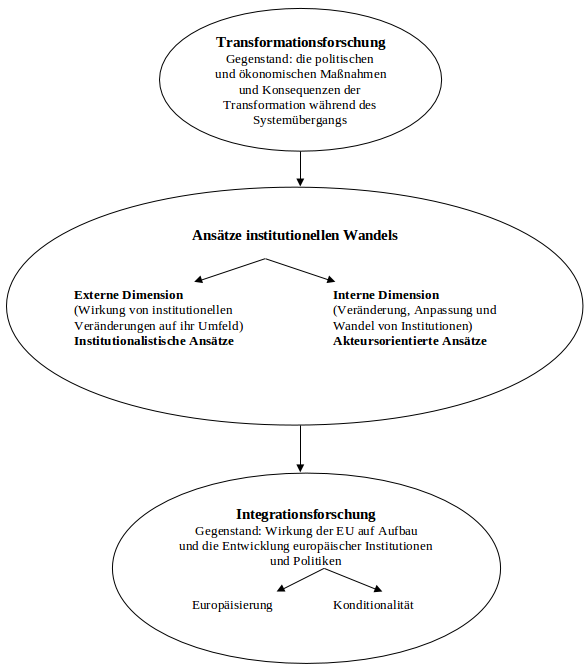
\includegraphics[width=5in]{Material/ForschungZuEuropUndKondi_ohneRand}\\

Quelle: in Anlehnung an \cite{huszak}: 75.
  \end{figure}
Erkennbar ist aus diesem Schema die Einbettung der Europäisierungs- und Konditionalitätsforschung in die übergeordneten theoretischen Konzepte Integrationsforschung, Forschung zu institutionellem Wandel und Transitionsforschung.\par
Moravcsik und Vachudova gehen von einer asymmetrischen Interdependenz zwischen Beitrittskandidat und der EU aus. Bei positiv verlaufender Konditionalität schätzen die Kandidatenländer die politischen Kosten der Anpassung ihrer nationalen Politiken niedriger ein als einen möglichen Ausschluss aus der EU und die damit verbundenen Nachteile (vgl. \cite{morvac}: 44).
\par
Schimmelfennig und Sedelmeier schlagen ein „external incentives“-Modell vor, das den Erfolg der EU-Konditionalität anhand von vier Faktoren beschreibt. Diese Faktoren führen dazu, dass nationale Regierungen EU-Regeln übernehmen, wenn die Vorteile größer sind als die Kosten der Anpassung. Die vier Faktoren sind “the determinancy of conditions, the size and speed of rewards, the credibility of threats and promises and size of adaption costs” (\cite{schsed05b}: 12). Angewandt auf die neuen EU-Mitgliedsländer kommen die Autoren zu dem Schluss, dass das „external incentives“-Modell von dem Typ der Konditionalität abhängt, wobei die Acquis-Konditionalität besser abschneidet als die politische Konditionalität (vgl. \cite{schsed05c}: 212). Die empirische Überprüfung führt zu dem Schluss, dass die Glaubwürdigkeit der Belohnung und die Höhe der politischen Anpassungskosten ausschlaggebend waren bei der Entscheidung der Anpassung an EU-Konzepte. Hinsichtlich der Glaubwürdigkeit erhöhte die Eröffnung von Verhandlungen die Wahrscheinlichkeit von nationalen Anpassungen, da sich damit in den Augen der Kandidatenländer der Wille der EU zeigte, die Verhandlungen auch zu einem Abschluss zu bringen (vgl. \cite{schsed05c}: 215). Weiterhin nimmt die Gefahr des Ausschlusses von der EU-Mitgliedschaft ab, je weiter der Assoziierungsprozess fortschreitet (vgl. \cite{dimit05}). Allerdings zeigte sich auch, dass hohe Anpassungskosten, die die Sicherheit oder Integrität des Staates oder das Überleben der Regierung gefährdeten, eine starke Behinderung darstellten, sogar bei glaubwürdigen Anreizen der EU. Nur im allerletzten Stadium der Verhandlungen („endgame“) haben die Staaten die Anpassungsleistungen vollzogen, sogar bei kurzfristigen hohen politischen Anpassungskosten im eigenen Land (\mbox{vgl. \cite{schetal}: 921}).\par

Huszka merkt in Bezug auf die Anwendung dieses „external incentives”-Modells auf den Balkan an: „However, while this ‘external incentive model’ according to which external rewards help elites to overcome domestic costs worked effectively in Central and Eastern Europe, its application to the Western Balkans is more problematic” (\cite{huszka}: 10). Hinzu kommt, dass die Mitgliedschaft für die in der vorliegenden Arbeit betrachteten Balkanstaaten noch stark in der Zukunft liegt. Daher sind die Belohnungen, die aktuell möglich sind, eher beschränkt.\par

Brusis konstatiert, dass demokratische Reformen verschiedene Ursachen haben und er geht davon aus, dass die Konditionalität der EU einen wesentlichen Einfluss hat, gibt aber auch zu bedenken: „Von der EU oder anderen externen Demokratisierungsakteuren gestellte Anforderungen sind aber weder a priori notwendige, noch hinreichende Bedingungen für innerstaatlichen Wandel“ (\cite{brusis05}: 298).

\subsection{Öffentliche Verwaltung und politische Konditionalität}

Die Notwendigkeit einer stabilen, effektiven und transparenten Verwaltung ist im Hinblick auf die Fähigkeit zur Übernahme des Acquis communautaire wichtig und wird in den Handreichungen der EU zur Übernahme des Acquis folgendermaßen formuliert: “A candidate country preparing for accession to the EU must bring its institutions, management capacity and administrative and judicial systems up to Union standards with a view to implementing the acquis effectively… At the general level, this requires a well-functioning and stable public administration built on an efficient and impartial civil service, and an independent and efficient judicial system” (\cite{eurcom05}: 7).\par
Die Existenz einer gut funktionierenden und stabilen öffentlichen Verwaltung ist eines der wesentlichen Kriterien innerhalb der EU-Konditionalität. Allerdings ist die öffentliche Verwaltung kein Kapitel des Acquis und unterliegt damit nicht der direkten Überprüfung anhand eines Kriterienkataloges. Die EU hat gemeinsame grundrechts- und allgemein rechtsstaatsbezogene Normen aufgestellt. Doch gibt es keine konkreten Vorgaben, wie demokratische Institutionen (Parlament, Regierung, Gerichte, Verwaltungsaufbau) organisiert sein sollen. Und in dieser Hinsicht existieren keine konkreten benchmarks, an denen sich die Beitrittsländer orientieren und deren Erfüllung man untersuchen könnte (vgl. \cite{brusis09}: 196). Von der EU wird das Thema Verwaltungsreform unter „politische Bedingungen“ behandelt und diese „politischen Kriterien“ nehmen einen festen Raum ein in den jährlichen Fortschrittsberichten der EU zu den Beitrittskandidaten.\par
Die Konditionalitätsforschung geht also von einem starken Zugzwang aus, in den die Kandidatenländer geraten, der dazu führt, dass sie die Anforderungen der EU zum Umbau ihrer nationalen Strukturen erfüllen. Dies wird deutlich im Rahmen der geforderten Übernahme des Acquis mit konkreten Kapiteln, die im nationalen Rahmen umzusetzen sind. Im Zusammenhang mit der Verwaltungsmodernisierung ist dies nicht so eindeutig nachvollziehbar, da es sich nicht um ein Kapitel des Erweiterungsacquis handelt.\par
Kennzeichnend für die Konditionalitätsforschung ist also die Konzentration auf die Frage, was die Veränderungen insbesondere in den Beitrittskandidaten befördert. Zentraler Gesichtspunkt sind dabei die Bedingungen der EU, die einem Beitritt vorausgehen, d.h. die Konditionalität. Im Kontext der vorliegenden Arbeit geht es hierbei insbesondere um die politische Konditionalität, unter die das Thema Verwaltungsmodernisierung fällt, ist kein Kapitel des Acquis und entfaltet daher vergleichsweise geringere Konditionalität. Dennoch wird die Struktur der Verwaltung und ihre Modernisierung bei den politischen Kriterien abgehandelt, wie z.B. in den jährlichen Fortschrittsberichten deutlich wird.\par
Insofern ist die Konditionalitätsforschung auch auf das Thema Verwaltungsmodernisierung in den Beitrittsländern anwendbar und kann wertvolle Hinweise liefern. \par
Im nächsten Abschnitt der Untersuchung werden deshalb die praktischen Aspekte der EU-Erweiterung, jeweils mit Rückbindung an das Thema Verwaltungsentwicklung und Verwaltungsmodernisierung, überblicksartig dargestellt. Es wird im weiteren Verlauf der Arbeit zu prüfen sein, welchen Stellenwert Verwaltungsmodernisierung für die EU im Zuge der Erweiterungsstrategie hat und wie Verwaltungsmodernisierung in der Erweiterungspolitik vorkommt.

% usw.
 
% Anhang*

\appendix
%\pagestyle{empty}
%\chapter{Questionnaire EU-officials, enlargement experts in the area of Public Administration Reform }
1. Which topics/areas are presently dealt with as a priority by the EU regarding Public Administration Reform in Albania/Macedonia and Montenegro? What are the developments you see there?

2. Do you think the EU approach regarding Public Administration Reform in Albania, Macedonia and Montenegro is adequate? Or should other aspects be included from your point of view?

3. Do you perceive differences in the EU approach compared with the experience with PAR during the last wave of enlargement?

4. The literature on enlargement sometimes argues with the legacy theory, in particular regarding the last wave of enlargement. Meaning that structures of previous regime set-ups have an influence on the present development of Public Administration Reform. What is your view on this issue regarding Albania/Macedonia and Montenegro?

5. How do you assess the cooperation within the EU Commission regarding Public Administration reform in Albania/Macedonia and Montenegro with the different Units, DG Enlargement, country desks, special PAR Unit and DG Admin? 

6. Public Administration Reform is not a separate chapter in the Acquis. Should it be a separate chapter? 

7. What is your take on the Treaty of Lisbon regarding Public Administration reform? Does the Lisbon Treaty lead to a different approach of the EU towards Public Administration Reform in the candidate and potential candidate countries? 

8. How do you asses the EU-Insturments to promote Public Administration Reform in Albania/Macedona and Montenegro as regards quantity and effectiveness:
Differentiate per country, if possible
CARDS (phased out)
Twinning
Twinning light
TAIEX
IPA
Did I forget to mention an instrument that is relevant?
9. Are these programmes well designed for the needs of PAR in Albania/Macedonia and Montenegro or do you perceive a need for adjustment in any of them? (Content or technical)


10. In your opinion, are there obstacles to PAR in Albania/Macedonia and Montenegro? And what would be necessary for successful PAR in Albania/Macedonia and Montenegro? 

11. Which other instituions/organizations or bilateral donors are important in regards to PAR in Albania/Macedonia and Montenegro? How do you asses their impact on PAR in the three countries? 

12. Who is responisble for co-ordinating the PAR activities of all the different donors in Albania, Macedonia and Montenegro and what is happening in this respect at the moment? 

13. Should the EU have additional or other priorities in future PAR programming in Albania, Macedonia and Montenegro. 

14. Is there anything else that is important in the context of my research that you would like to comment on?
%\chapter{Questionnaire Public Administration Reform experts in Albania, FYROM, Montenegro}

1. Which main topics/areas in the context of Public Administration Reform are presently dealt with as a priority by Albania/Montenegro/FYROM?

2. Is the institution/structure dealing with PAR adequate for the tasks ahead? 

3. In your opinion, are there obstacles to PAR in Albania/Macedonia and Montenegro? And what would be necessary for successful PAR in Albania/Macedonia and Montenegro? 

4. Public Administration Reform is not a separate chapter in the Acquis. Should it be a separate chapter? 

5. How do you assess the cooperation within the EU regarding Public Administration Reform in Albania/Macedonia and Montenegro 

6. Do you think the EU approach regarding Public Administration Reform in Albania, Macedonia and Montenegro is adequate? Or should other aspects be included from your point of view?

7. What is your opinion, how does the new IPA instrument work for PAR in Albania, Montenegro and Macedonia? Examples?

8. Is this programme well designed for the needs of PAR in Albania/Macedonia and Montenegro or do you perceive a need for adjustment ? (Content or technical)

9. Which other institutions/organizations or bilateral donors apart from the EU are important in regards to PAR in Albania/Macedonia and Montenegro? How do you asses their impact on PAR? 

10. Who is responsible for co-ordinating the PAR activities of all the different donors in Albania, Macedonia and Montenegro and what is happening in this respect at the moment? 

11. Should the EU have additional or other priorities in future PAR programming in Albania, Macedonia and Montenegro. 

12. Is there anything else that is important in the context of my research that you would like to comment on?
%\begin{landscape}
\chapter{Übersicht über durchgeführte Interviews}
\label{Übersicht über durchgeführte Interviews}
 \renewcommand{\arraystretch}{1.5} 		
\begin{table}[!hbt]\vspace{1ex}\centering		
\begin{tabular}{|l|l|l|l|l|}\hline
Kennung im Text&Datum&	Zeit&	Ort Interview\\\hline\hline
EC Official, DG ELARG PAR Coordination team&17.09.2010&10:30-12:00&Europäische Kommission, Brüssel\\
OECD/SIGMA team&13.09.2010&12:00-13:30&OECD, Paris\\
EC Official, DG ELARG Evaluation Unit team&	15.09.2010	&9.00-10.00&	Europäische Kommission, Brüssel\\
EC Official, DG ELARG Albania team&	16.10.2010	&17:00-17:30	&Europäische Kommission, Brüssel\\
EC Official, DG ELARG Macedonia team&	15.09.2010	&10:30-11:30&	European Commission, Brüssel\\
EC Official, DG ELARG Montenegro team&	05.10.2010&	15:00-16:00&	Europäische Kommission, Brüssel\\
Official Albania&	17.01.2011&	8:30-09:30	&Department of Public Administration, Tirana\\
NGO Representative Albania	&17.01.2011&	16:00-17:00	&Büro der NGO, Tirana\\
Official Macedonia	&15.01.2011&	11:00-12:00&	Büro der Civil Servants Agency, Skopje\\
NGO Representative Macedonia	&15.01.2011	&13:00-14:00	&Büro der NGO, Skopje\\
Official Montnengro	&19. 1. 2011&	10.00-11.00&	Finanzministerium, Podgorica\\
NGO Representative Montnegro	&19.01.2011&	16:00-16:45&	Hotel, Podgorica\\\hline
\end{tabular}
	\end{table}	
	\end{landscape}	

%\begin{landscape}
\setlist{nolistsep}
\setitemize{noitemsep,topsep=0pt,parsep=0pt,partopsep=0pt,nolistsep,leftmargin=*,label={}}
\chapter{Vier zentrale politisch-administrative Traditionen}	
	
\renewcommand{\arraystretch}{1.4} 
\begin{table}[!hbt]\tiny
\begin{tabular}{|L{4cm}|L{5cm}|L{5cm}|L{5cm}|L{5cm}|}\hline
&\textbf {\footnotesize Deutsch}&	\textbf{\footnotesize Französisch}&\textbf {\footnotesize Angelsächsisch}&	\textbf{\footnotesize Skandinavisch}\\\hline
Verhältnis Staat-Gesellschaft&	organisch&	antagonistisch&	pluralistisch&	organisch\\\hline
Politische Organisation&föderalistisch&zentralistisch	&begrenzt föderalistisch&dezentralisiert, unitaristisch\\\hline
Politikstil&	legalistisch	&korporatistisch, legalistisch&	inkrementell&	konsenuell, technokratisch\\\hline
Dezentrale Elemente&	kooperativer Föderalismus&	regionalisierter Einheitsstaat&	State Power (US), Local Government (UK)&	starke lokale Autonomie\\\hline
Vorherrschende Sichtwiese auf öffentliche Verwaltung&	Öffentliches Recht	&Öffentliches Recht&	Politische Wissenschaft/ Soziologie	&Öffentliches Recht (SWE), Organisationstheorie (NO)\\\hline
Historische Dimension&	Preussische Tradition	&Napoleonische Tradition&	Civic culture Tradition&	Wohlfahrtsstaatsmodell\\\hline
Legale Basis der öffentlichen Verwaltung
&
\begin{itemize}
\item gesonderte Gesetze zu öfentlichem Dienst
\item Verfassungsstatus des öffentlichen Dienstes
\end{itemize}
&
\begin{itemize}
\item gesonderte Gesetze zu öfentlichem Dienst            
\item negative Definition öffentlicher Verwaltung 
\end{itemize}
&
 \vspace{-2mm}
\begin{itemize}
\item gesonderte Gesetze zu öfentlichem Dienst
\item keine Verankerung des öffentlichen Dienstes in der Verfassung
\item Rolle der öffentlichen Verwaltung eher in dienenderer Tradition als in Kontinentaleuropa
 \vspace{-2mm}
 \end{itemize}

&
\begin{itemize}
\item gesonderte Gesetze zu öfentlichem Dienst            
\item Mischung aus Deutschem und Angelsächsischem Modell
\end{itemize}\\\hline
Grad der Zentralisierung&
\begin{itemize}
\item vertikale und horizontale Fragmentierung
\item administrative Dezentralisierung
\item hierarchische Strukturen
\end{itemize}
&
\begin{itemize}
\item unitaristische und stark zentralistische Regierung und öffentliche Verwaltung
\item hierarchische Strukturen
\end{itemize}
 &
\begin{itemize}
\item unitaristische und zentralistische politisch-administrative Strukturen
\item wenig hierarchische Strukturen 	
\end{itemize}
&
Mischung aus Deutschem und Angelsächsischem Modell\\\hline
Koordination innerhalb der öffentlichen Verwaltung	&inter-minsterielle Koordination	&begrenzte inter-ministerielle Koordination&	inter-minsterielle Koordination&	Mischung aus Deutscher und Angelsächsischer inter-ministerieller Koordination\\\hline
Administrativer Rahmen	&
 \vspace{-2mm}
\begin{itemize}
\item einheitlicher administrativer Rahmen auf allen Ebenen
\item föderaler Rahmen mit regional und kommunalverwaltung
\item unterschiedliche Sub-Verwaltungen mit eigenen Kompetenzen
\item vertikale Verteilung von Kompetenzen zwischen den verschiedenen föderalen Ebenen
 \vspace{-2mm}\end{itemize}

&
\begin{itemize}
\item einheitlicher administrativer Rahmen
\item administrative Untereinheiten direkten Weisungen der Zentralregierung unterstellt
\item strikt zentralistische Orientierung
\end{itemize}
&
\begin{itemize}
\item weitgehend autnomome Exekutiv Organe
\item untergeordnete administrative Einheiten mit eingeschränkter finanzieller Autonomie           
\end{itemize}
&
\begin{itemize}
\item zentralistischer Aufbau
\item Mischung aus Deutschem und Angelsächsischem Modell
\end{itemize}\\\hline
Verhältnis von Politik und öffentlicher Verwaltung&	Trennung von öffentlicher Verwaltung und Politik&
\begin{itemize}
\item Trennung von öffentlicher Verwaltung und Politik
\item enge Beziehungen zwischen Politikern und Verwaltern
\end{itemize}
&
 \vspace{-2mm}
\begin{itemize}
\item civic culture und individualistische Tradition
\item Trennung von öffentlicher Verwaltung und Politik
\item Werte des politischen Systems bestimmen auch die öffentliche Verwaltung
 \vspace{-2mm}
 \end{itemize}

&	Mischung aus Deutschem und Angelsächsischem Modell\\\hline
Personalpolitik und Rekrutierung&
\begin{itemize}
\item Primat von Universitätsausbildung im höheren Dienst
\item Hauptsächlich Juristen
\item Beamte sind der personifizierte Staat
\item Ernennung aufgrund von Qualifikation und Leistung, mit begrenzten politischen Ernennungen (höhere Positionen)
\item Lebenszeit und Staatsbediensteten auf Vertragsbasis	
\end{itemize}&
 \vspace{-2mm}
\begin{itemize}
\item vorwiegend administrative Elite
\item hauptsächlich Juristen, aber auch Generalisten
\item homogene mentale und kognitive Übereinstimmung der Bediensteten in der Verwaltung                             \item Rekrutierung vor allem aus spezialisierten Verwaltungsschulen
\item Ernennung aufgrund von Qualifikation und Leistung, mit begrenzten politischen Ernennungen (höhere Positionen)
\item Karriereorientierung
 \vspace{-2mm}
\end{itemize}
&
\begin{itemize}
\item kein Einfluss von Politikern auf Beförderung
\item Universitätsausbildung für höhere Positionen
\item  vorwiegend Generalisten
\item Bestimmte Universitäten bei der Rekrutierung bevorzugt
\item Karrieresystem
\end{itemize}&	Mischung aus Deutschem und Angelsächsischem Modell\\\hline
Länder&	Deutschland, Österreich, Niederlande, Spanien (nach 1978), Belgien (nach 1988)&	Frankreich, Italien, Spanien (bis 1978), Portugal, Griechenland, Belgien (bis 1988) 	&UK, US, Irland&	Schweden, Norwegen, Dänemark\\\hline
\multicolumn{5}{l}{}
\multicolumn{5}{l}{nach Loughlin (1994) aus: \cite{lipumb05} :65ff}
\end{tabular}
\end{table}	

\end{landscape}	

%\pagestyle{myheadings} 
%\pagestyle{empty}
\chapter{Questionnaire EU-officials, enlargement experts in the area of Public Administration Reform }
1. Which topics/areas are presently dealt with as a priority by the EU regarding Public Administration Reform in Albania/Macedonia and Montenegro? What are the developments you see there?

2. Do you think the EU approach regarding Public Administration Reform in Albania, Macedonia and Montenegro is adequate? Or should other aspects be included from your point of view?

3. Do you perceive differences in the EU approach compared with the experience with PAR during the last wave of enlargement?

4. The literature on enlargement sometimes argues with the legacy theory, in particular regarding the last wave of enlargement. Meaning that structures of previous regime set-ups have an influence on the present development of Public Administration Reform. What is your view on this issue regarding Albania/Macedonia and Montenegro?

5. How do you assess the cooperation within the EU Commission regarding Public Administration reform in Albania/Macedonia and Montenegro with the different Units, DG Enlargement, country desks, special PAR Unit and DG Admin? 

6. Public Administration Reform is not a separate chapter in the Acquis. Should it be a separate chapter? 

7. What is your take on the Treaty of Lisbon regarding Public Administration reform? Does the Lisbon Treaty lead to a different approach of the EU towards Public Administration Reform in the candidate and potential candidate countries? 

8. How do you asses the EU-Insturments to promote Public Administration Reform in Albania/Macedona and Montenegro as regards quantity and effectiveness:
Differentiate per country, if possible
CARDS (phased out)
Twinning
Twinning light
TAIEX
IPA
Did I forget to mention an instrument that is relevant?
9. Are these programmes well designed for the needs of PAR in Albania/Macedonia and Montenegro or do you perceive a need for adjustment in any of them? (Content or technical)


10. In your opinion, are there obstacles to PAR in Albania/Macedonia and Montenegro? And what would be necessary for successful PAR in Albania/Macedonia and Montenegro? 

11. Which other instituions/organizations or bilateral donors are important in regards to PAR in Albania/Macedonia and Montenegro? How do you asses their impact on PAR in the three countries? 

12. Who is responisble for co-ordinating the PAR activities of all the different donors in Albania, Macedonia and Montenegro and what is happening in this respect at the moment? 

13. Should the EU have additional or other priorities in future PAR programming in Albania, Macedonia and Montenegro. 

14. Is there anything else that is important in the context of my research that you would like to comment on?
%
\chapter[Interview with EU-officials, enlargement experts]{Interview with EU-officials, enlargement experts in the area of Public Administration Reform}
\label{anhang:InterviewEuOfficials}
%---------------------------------------------------------------------------------------------------------------------------
\section{Which topics/areas are presently dealt with as a priority by the EU regarding Public Administration Reform in Albania/Macedonia and Montenegro? What are the developments you see there? }
\label{sec:there}

\markboth{Anhang \thechapter, Frage Nr. \thesection}{Anhang \thechapter, Frage Nr. \thesection}
\textbf{EC official, DG ELARG PAR Coordination team}: PAR, or governance is a key priority in the enlargement process. The updated partnership documents with each country, list the priorities, which might differ from country to country. Mostly priorities related to PAR are found under political criteria and there we have them under Parliament, Government and PA, but also under headings such as civil and political rights and anti-corruption and possibly under chapter 23 Judiciary and Fundamental rights or chapter 32, financial control, some of these functions can also be seen as part of the horizontal PA tasks. The main priority in all the countries is to establish a civil service and a PA that is professional and not influenced by political constellations. There is a tendency, especially after elections to replace many people in the PA. We should distinguish between changes in the legislation related to the public administration and to make them conform with what we call European standards. The other point is implementation and enforcement of those laws. But I must say, in both areas, progress is usually slow. And even when good laws are enacted, you often do not find the administrative capacity in these countries to implement them or the political will. \\
\textbf{OECD/SIGMA team}: There is a tendency to understand PA in terms of civil service and administrative law and to some extent policy making, lately. For PA, we think, this is too narrow. It should be Public Governance. If you are dealing with PA, it should be wider than 3 or 4 main topics. Within the EU's definition of PA in the three countries, there is a strong interest in PAR-Strategies, in Montenegro and Macedonia and perhaps a bit less so in Albania, and in that the main focus tends to be on civil service law and anti-corruption. Lately, there is increasing interest in Admin Procedures and Admin Justice.\\
\textbf{EC official, DG ELRG Evaluation Unit team}: One of the goals is to install democratic stability in these countries with functioning institutions. The institutions we focus on are very much in the sector Justice and Home Affairs and institutions linked to democratic stability. Quite a few of the PAR projects focus on institutional structures and their ability to implement community law. Not in all of the countries we are using all of the instruments. In Montenegro, we are not using Twinning as heavily as in Albania, for example. Twinning is very helpful if you have counterparts in the host country administration. If you do not have that, the results of the projects can be in question. Montenegro is a small country with fewer and smaller institutions and right now, they are very much stretched with their engagement in the pre-accession process. And we know that from the past, even for Slovenia that this is always an extra strain on a small country. So, of course we are careful not to force too many heavy projects on them. \\
\textbf{EC official, DG ELARG Macedonia team}: The main topic now is related to civil service law and that is the topic of recruitment, the principle of recruitment based on merit and on a transparent process. We also saw overuse of so called temporary employments, which might be a specific case for Macedonia. The state administration for whatever capacity they needed would get staff through private employment agencies for one year on a short term contract to do the job of a civil servant. In summer 2010, the authorities of Macedonia started the process of recruitment and there are indications that not everything was as transparent as it should be. And there are signals that those who were temporarily employed were given an advantage, if they were not directly transferred, which is of course against the principles. There is a Civil Service Agency (CSA) as a body independent from the government and reporting to Parliament. In reality, this arrangement has also created some problems, because for many they are just an agency. So you can imagine that a ministry of finance would hardly listen to someone from an agency telling them how they should do their work. Macedonia is now preparing an updated national PAR strategy, the first update in 10 years. And we understand there is the plan to have a ministry for PA. So the current Ministry for IT will be combined with Ministry for PA. Then the CSA would be included in the organization of this ministry as one of the departments. \\
\textbf{EC official, DG ELARG Albania team}: PAR is an overarching horizontal aspect that goes beyond the political criteria, but that is reflected specifically in the political criteria and PAR is an issue for Albania. We analyze the current situation and we give our view. In our view PAR in Albania is incomplete; there are certain issues we are following up very closely and in detailed discussions and exchanges with SIGMA. We are fully in line with the analysis SIGMA is providing in this regard on the ongoing process of civil service law reform in Albania and strengthening the department that deals with that reform. These are priorities for us in terms of financing.\\
\textbf{EC official, DG ELARG Montenegro team}: Priorities are mainly in the filed of civil service, training issues and the non-political recruitment of civil servants in every ministry. Non political civil servants still needs to improve in Montenegro. A Human Resources Management Agency was created, but unfortunately it is not yet in the lead on reforms. A person in the Deputy Prime Minister's Office has been nominated as the central contact point for PAR. There is a new PAR strategy named AURUM. For 2011, the EU foresees a large IPA project for PAR in Montenegro. In all the WB countries the main IPA projects deal with are in the realm of Rule of Law/Good Governance and PAR. \\
%%\newpage
%---------------------------------------------------------------------------------------------------------------------------
\section{ Do you think the EU approach regarding Public Administration Reform in Albania, Macedonia and Montenegro is adequate? Or should other aspects be included from your point of view? }
\label{sec:view}
\markboth{Anhang \thechapter, Frage Nr. \thesection}{Anhang \thechapter, Frage Nr. \thesection}
\textbf{EC official, DG ELARG PAR Coordination team}: The discussion is what comes first, legislation or culture. You can say that culture is affected by the laws and by enacting new laws, good laws you can influence and bring about change in a country. Another approach is based on trying to draft strategies for change, listing the objectives, and having an action plan with everything carried out according to that plan. But it did not always work like that. Maybe the strategies themselves were not professional. Maybe important elements of a strategy were missing, like a clear definition of the objectives and a realistic, continuously monitored action plan. Sometimes, the scope of PAR and governance were not defined. There is no dedicated Acquis chapter on PAR and thus, no framework for discussions. Fortunately, there seems to be growing awareness, even without Acquis. And in the case of Macedonia, there is a new  high-level working group on PAR. Also checks and balances are very important. Institutions to deal with complaints against the public administration or the government, reform of the ombudsperson institution, but also external audit with Supreme Audit Institutions. According to international standards, a supreme audit should also carry out performance audits of government programmes and activities. While this is just starting for some of these countries, it will contribute to the reform in PA. \\
\textbf{OECD/SIGMA team}: The scope of PAR should be widened to include financial aspects and policy aspects and to focus on results rather than on inputs. What we have been doing in the past and the Commission has been doing in the past is worrying more about who makes a decision than about the decision itself. The other aspect is, not seeing PA as independent from its governance context. Thus, I think that civil service reform is not appropriate to the context. Civil service reform, professionalizing and depoliticizing the civil service, at the moment is a xeno-transplant which will suffer pathological rejection. The second point is that the EU is pushing countries to reform all the time and this is substituting the presence of a reform programme for administrative performance. I think much greater emphasis has to be on the idea of implementing previous policies and previous laws and not pushing people to continuous reforms. This results in diverting resources to perform reform activities away from implementing activities. Lastly, I think that adequacy includes the quality aspect and there is a lot to be said about the quality of support given to the countries for PAR, which is largely driven by the technical assistance with management systems that have been adapted.\\
\textbf{EC official, DG ELARG Evaluation Unit team}: We are at the moment looking at the way we programme accession funds. One of the things we are thinking about is to introduce the sector wide approach, to put the focus on certain priority sectors over a period of three years. The MIPD will be the main document driving this reform, to enable us to focus on priority sectors in the countries. Evaluations of previous enlargement rounds suggest that we maybe covered too much ground at once and the countries found it difficult to prioritize between the different sectors. When MIPDs are drafted, there is a discussion on how to determine the priority sectors with the Delegations and the countries and of course this is linked to the progress reports, accession partnerships and all the top level documents. Some countries came up with a list of three, others with a list of ten priority sectors. These proposals are now being discussed, we have until January (2011). The idea is not only to have sectors, but you also ask countries to have a strategy for each of the sectors. The strategies will be linked to a budget. It is not only us putting money in; it is also the national budget of the countries and the donors that contribute to these sectors. We would end up, let us say, with a set of eight priority sectors and then the countries in cooperation with the Delegations decide which sectors should be covered by which donor.\\
\textbf{EC official, DG ELARG Macedonia team}: I think in our case and also due to the fact that we are the first ones to have this special platform for Macedonia exclusively dedicated to PAR, we took a comprehensive approach. We really want to discuss all aspects of PAR, starting with the basic institutional framework, but looking also into aspects like corruption and transparency as well as donor coordination. It should really be a forum for everything that relates to PA to be discussed. Maybe not everything to the same detail, because we have other fora, such as on corruption and we have a sub-committee on Justice and Home Affairs. But we can talk about prevention and the organizational side more in our special group. This still has to be fine tuned, but we really try to be comprehensive and see PAR as an across the board issue, which is somehow related to many areas of the Acquis.\\
\textbf{EC official, DG ELARG Albania team}: We see PA as overarching and horizontal responsibility because it relates to the question of the foundation of the state, of having good governance, stable institutions and a civil service with the right competences, professionalism and ethics. But we do not have a special programme other than this general wish for good governance. We have PAR as part of the political criteria, which have to be sufficiently met for a country to start negotiations. In that respect, early attention to good governance and setting priorities that have to be met could be seen as approach. We also give it attention in financial assistance; we have the IPA instrument for preaccession assistance. The strong cooperation with OECD/SIGMA is another sign that we want to go into depth in the analysis, in order to find the areas that need to be targeted with advice or assistance. Regarding a definition of PAR, I think we are generally inspired by SIGMA. And we try to adapt it as much as 
possible to our client countries.\\
\textbf{EC official, DG ELARG  Montenegro team}: Montenegro is a special case. Reports mention the poor administrative capacity, but it does have an administration that corresponds to the size of the country. The EC is working on analyzing the specific needs of small countries together with SIGMA. Some EU requests might have to be adjusted to the size of the country, we hope for a new and innovative approach in that respect. For example we had discussion on the advantages of long term TA over  short term assistance in the long term: i.e. the same person coming for one week per month during two years for example. With TA however, sometimes dependency on one foreigner for a long time is the case. When this person leaves, the momentum drops ! Maybe short term consultants will keep the momentum up? SIGMA is more in favour of short term and flexible approaches. TAIEX is a short term assistance focussing on the EU Acquis, it is very efficient.\\
%\newpage
%---------------------------------------------------------------------------------------------------------------------------
\section{Do you perceive differences in the EU approach compared with the experience with PAR during the last wave of enlargement? }
\label{sec:enlargement}
\markboth{Anhang \thechapter, Frage Nr. \thesection}{Anhang \thechapter, Frage Nr. \thesection}
\textbf{EC official, DG ELARG PAR Coordination team}: Yes, as a conclusion from the last wave, we issued a renewed consensus in our enlargement strategy that was issued and adopted in 2006. We focus on a stricter conditionality in all phases of the process, because we realized that in the previous enlargement rounds, we were not as strict as we should have been perhaps, in particular with these two countries that became members in 2007. We also realized that we need to address difficult issues, not only when it comes to judicial reforms, but PAR in general and the fight against corruption much earlier in the enlargement process. This message has been repeated in the following enlargement papers. In the last one for 2009, there was even a special section dedicated to the rule of law. And under a heading 'bringing the citizens and administration closer to the EU', the Commission stated that it will continue to pay close attention to the existence of a professional and functioning PA in line with the focus on basic governance issues. \\
\textbf{OECD/SIGMA team}: There are differences, yes. The last wave of enlargement was driven by a time pressure, which had to do with geopolitical concerns, not with EU-readiness concerns. Time pressure forced people to do things very differently, for example, there was a much greater focus on key risk areas for the internal market. There was a greater focus on sectoral administrative development, and a lesser focus on systemic issues. That is absolutely not a criticism. As for the 8 CEECs, the timing was driven by real valid concerns, which was not the case for Bulgaria and Romania, but unfortunately, the freedom of that not being the case was not used. The Balkans present very different problems; first of all, it is a post-conflict setting. There are large numbers of ethnic and state issues, which are unresolved. Most countries in the Balkans have rather weak states and national (as opposed to ethnic) identities; this was not the case in the CEECs. And the Balkans have weak state institutions with the possible exception of Serbia. So these countries have made very rapid progress, but the institutions of state are still rather weak, and democratic culture and the rule of law culture have not fully been internalized. I do not think the Commissions assistance either in terms of its prioritization or in terms of its delivery mechanisms have been sufficiently adapted to these circumstances. \\
\textbf{EC official, DG ELARG Evaluation Unit team}: Of course, if you look at PAR, the issues are very much the same, but the underlying issues are different. For example, if you have a country like Albania, where the administration is constantly changing when parties in power change, not just in key positions, it is very difficult to operate or start a change process. What I do not see so much in these countries as opposed to the last wave of enlargement are parties that are in opposition of the EI. They do exist, but not in large numbers. So, the main forces in the countries are pro-European. But of course you still have a quite politicized civil service, which is the problem. In the Balkans the general feeling is that the EI-process has to stabilize the region, which in practical terms it is a completely different process than in Eastern Europe. Right now, there is a discussion about looking at these countries not so much already as accession countries, but also as countries in development. And if you read the IPA regulations, it is explicitly stated there that development should be a key part in potential candidates. I don't think that we actually reflected on that enough. We just took instruments like Twinning and Twinning light, TAIEX, etc. and we are just now really adapting them, adapting them fully or revising some of the instruments.\\
\textbf{EC official, DG ELARG Macedonia team}: I think there are a lot of lessons learned. There are similar problems with several countries of the last wave of enlargement. And I think it is due to the lessons learned, why there is this idea of a specialized dialogue on PAR. What we saw before the discussion on PAR was just based on political criteria. Once these political criteria were fulfilled, there was not really a follow up. SIGMA conducted a study on the situation in the countries, which recently joined the EU and their finding is that there was a lot of backsliding in the PA regarding adherence to principles etc. It was quite evident that PA, although it is very important, it is sort of difficult to pinpoint where the boundaries are, so it is not really followed up. With this new approach, what we are trying to do is to have a regular dialogue, where we could really see from one month to another, what really happened. And even when the political criteria are fulfilled and a country received recommendations for opening negotiations, you can still have a place where you can raise issues. In the last wave of enlargement there was no forum to continually look at PA issues after negotiations started. \\
\textbf{EC official, DG ELARG Albania team}: I think in general, yes. This is also a general comment on the political criteria. Of course we have learnt our lessons from the fifth enlargement. We are at an earlier stage addressing certain issues and that includes of course the rule of law, corruption and organized crime. Within this, it is also about governance in these institutions. And also, we do now establish certain targets that need to be reached before we start negotiations. You can see this already in Macedonia, not immediately the opinion, but what was published shortly after. The opinion itself does not give key priorities, but the accession partnership or European partnership do. For Macedonia we have the opinion 2005, and in 2008 we have the updated accession partnership with key priorities that need to be fulfilled before the country can start negotiations. This is a model that could be pursued, which is presently discussed. The philosophy in any case is there. We will want to see the issues addressed at a much earlier stage, even before negotiations start and that could include the priority on public administration.\\
\textbf{EC official, DG ELARG Montenegro team}: There is not really a different approach. But now, PAR is high on the agenda. PAR includes a vast area of topics. It relates not only to the services provided, but also for example to the structures in each ministry. In June 2008, a National Action Plan for Integration (NPI) was designed for implementing the SAA, which is very comprehensive. The NPI will be revised after the opinion on Montenegro will be published. \\
%\newpage
%---------------------------------------------------------------------------------------------------------------------------
\section{The literature on enlargement sometimes argues with the legacy theory, in particular regarding the last wave of enlargement. Meaning that structures of previous regime set-ups have an influence on the present development of Public Administration Reform. What is your view on this issue regarding Albania/Macedonia and Montenegro? }
\label{sec:montenegro1}
\markboth{Anhang \thechapter, Frage Nr. \thesection}{Anhang \thechapter, Frage Nr. \thesection}
\textbf{EC official, DG ELARG PAR Coordination team}: Obviously, there is a common legislative background in all the former Yugoslav countries, when it comes to civil service, which is of course not in line with European standards. And also, unfortunately, when these countries became potential candidate countries, we asked them to reform their legislation, it seems to me that they have been using sometimes experts, who themselves had been brought up under that legislative background. So when it comes to certain legislation of civil service continued to amend those laws in line with those old values, so to say. Obviously those structures or set-ups or values had an influence on the present development. \\
\textbf{OECD/SIGMA team}: The recent Sigma paper No. 44 on civil service reform in the CEECs after accession, does not very much support the legacy theory. But intuitively, the legacy theory must mean something. Probably what the legacy theory does not predict in the CEECs is the differences. But if you take legacy as very basic concept, with these countries starting from a communist system of governance and then switching to a democratic, market oriented, rule of law one, then the legacy theory is an underlying idea, which we have to take into consideration all the time. I think legacy theory in the Balkans is very important, but legacies are different. For example in Serbia and Montenegro, the sanctions regime and the way the states were forced to operate under the sanctions, have an enduring effect. In Albania it is necessary to keep in mind, the harshness of the regime before compared to what was happening in the rest of the Balkans. The rest of the Balkans were relatively open, whereas Albania was totally closed. 16 years on, the legacies are still there in people's mentalities. They are still there in people's understanding of law, both citizens and power elites. And power elites still understand themselves as the architects of law, but not the subjects of law. Now, some of that goes back to pre-communist legacies. That takes you into the area of social, cultural explanations, which is very, very difficult to handle. You have the Austrian/Turkish legacy, we have the communist legacy and we have the post-communist legacy, because after all it is now 20 years after the wall fell. Some of these countries then went through conflict, some of them were under regimes like those of Milosevic and Tudjman, which introduced their own legacies into the system and which stay on in terms of criminal networks and oligarchic arrangements. So, as I said legacies are a very complicated topic. I think you can talk about a sort of substrate, but I think it is very difficult to use legacies for identifying differences. \\
\textbf{EC official, DG ELARG Evaluation Unit team}: There is of course a certain culture in PA and there is the civil service code. But of course what happened after the overthrow of the communist regimes, all of this has been just filed away and it was built up from scratch. A very interesting research question would of course be to compare the old and the new civil service code and see how much of it actually matches. That is a big question how much of the old traditions have carried over into the 'new' institutions. There is a certain mentality. We are mostly dealing with administrations that are stretched to the limit; I am hearing that mostly from our colleagues in the country units. Do not ask them for too many things, because they just do not have this capacity. For example now, we want to organize a training for evaluation and monitoring and just to get the commitment for one training day for maybe 10-12 people, it is almost like shutting down the whole ministry. Especially in Kosovo and Montenegro. Of course we have to take that into account. \\
\textbf{EC official, DG ELARG Macedonia team}:. I think yes. It goes back to the Austro-Hungarian Empire, some of the principles that are embedded in their laws. The law on Administrative Procedures you can trace this back a very long way. The Austro-Hungarian Empire was encompassing countries which were later on transition countries and you could see similar issues or problems in the way to approach things, the heritage, also in the Czech Republic, Slovakia, Hungary and now in the Balkans. While Macedonia never was part of the Austro-Hungarian Empire, it inherited from Yugoslavia, which was heavily based on the older model. So, that is how we can trace the heritage. The country was heavily influenced by the set up of the administration, education and the entire package of Yugoslavia and that is of course why you can see some of the same problems in Croatia, Montenegro and elsewhere in the region. \\
\textbf{EC official, DG ELARG Albania team}: More than a legacy in the structure, there is a legacy in the culture. In Albania probably more so than in any other country. You have a legacy of respect of the highest authority being the only institution that can change things. Although you have that in all ex-communist countries, you have that very strongly still in Albania. So, it is culture more than structures, I would say.\\
\textbf{EC official, DG ELARG Montenegro team}: Until 1989 most of the countries of the last wave of enlargement had central planning. For the Balkan countries the situation is different, as these countries have had the time to start the needed changes. We are much further on in time and also the structure of the state was different than in most of the countries of the last wave of enlargement. In addition, there were wars in the Balkan countries as opposed to the countries of the last wave of enlargement. It is extremely important that these countries talk to each other. Two years ago the DG RTD1 produced a good study based on ethnic research and said among many interesting findings, that we should be careful not to create "ethnocracies".\\
%\newpage
%---------------------------------------------------------------------------------------------------------------------------
\section{How do you assess the cooperation within the EU Commission regarding Public Administration reform in Albania/Macedonia and Montenegro with the different Units, DG Enlargement, country desks, special PAR Unit and DG Admin? }
\label{sec:admin}
\markboth{Anhang \thechapter, Frage Nr. \thesection}{Anhang \thechapter, Frage Nr. \thesection}
\textbf{EC official, DG ELARG PAR Coordination team}: There is very close cooperation within DG Enlargement. There is dedicated country desk for each country and the Delegations in each of the countries. We have the coordination unit both for the political side for producing the annual progress reports, which is unit A1, and unit D1 for the instruments and contracts, which is responsible for correct application of the financial instruments, especially the IPA-Instrument. Take for example financial assistance, there unit D1 regularly organizes meetings, here in Brussels mostly, with the heads of the operational sections in the Delegations. They are constantly kept updated on everything here. There are a number of PAR IPA-projects in each country. IPA projects do not need to be linked to an Acquis chapter; they can also target political criteria. There is a long programming-process, where all the stakeholders, first of all the national authorities themselves, then the Delegations are involved. One important new element in the whole process was when DG Enlargement about three years ago established a so called quality support group (QSG) where drafts of project fiches, which later will be part of the annual national programmes of the countries are discussed quite in detail and are circulated in various units. The aim is to ensure that we plan projects with IPA-support for those areas where we find gaps, where there is a need for reform or a need for institution building. Overall, there are people responsible for financial assistance and others more responsible for the political dialogue. \\
\textbf{OECD/SIGMA team}: We need to make a clear distinction between the political discourse and negotiations on one hand and technical assistance on the other hand, which in my opinion are not always connected, posing something of a problem. The Brussels-based country desks do try to keep the TA part linked to the negotiations. But the TA part tends to be driven by disbursement issues and the Delegations. In DG Enlargement, I think it is fairly tightly connected and to some extent the requirement to produce the regular reports and the multi-annual programming, drives the cooperation process and similarly with the other DGs. With the Delegations, there seem to be two separate issues. One between Delegations and HQ, which will become at least more complex with the arrival of the External Action Service and the other, is the relations in the Delegations between the operational and the political units, where I think coordination could be quite significantly improved. DG Enlargement relies very heavily on external experts and neither DG enlargement nor the Delegations seem to have the technical abilities to steer/control all the technical assistance they are producing. Technical assistance is managed at the administrative contract level and not really at the substance level and the substantive dialogue with countries does not really take place. \\
\textbf{EC official, DG ELARG Evaluation Unit team}: There are several processes and everything we do is cooperation between the units. We want to use the evaluation unit more regarding the question of lessons learned of all the evaluation reports. One question that always is difficult for consultants or our evaluations to answer is on impact and sustainability, based on the five OECD criteria: relevance, efficiency, effectiveness, impact and sustainability. It is quite hard to come to a judgement, if you do not have some sort of a basis. You have to know what was there at the end of a project. Otherwise it is hard to judge what is still there in a year or two years after. With the sector approach there is leverage. You basically ask for a strategy and commitment to certain objectives in the strategy. Things are then formulated out in national programmes and projects. With these projects you can then say, now tell us why you want this project and how does it contribute to your strategy in the Justice sector, let us say. It is all linked up in a logical sequence towards accession. We will most likely have better donor cooperation, more targeted and sequenced funding for assistance and that has of course a large effect for PAR as well.\\
\textbf{EC official, DG ELARG Macedonia}: We have a system of so called chapter desks. For every chapter of the Acquis, like agriculture or fisheries, you have someone in DG Enlargement, who is getting the overview of all countries on that chapter. Somebody will be dealing with Albania, but there is also somebody looking at a chapter in all the countries. This is to make sure there is consistency of approach. We did not have anybody specifically for PAR as it is not a chapter. SIGMA is sub contracted to do work on PA, as we do not have the capacity. For the time being, I am in touch with DG HR, SIGMA, the PAR Coordinator and DG Justice, as DG Justice is the one dealing with aspects of corruption for example. I am in touch with DG Budget on issues of Public Finance and DG Market on public procurement, even with OLAF on issues of anti-fraud. So, because there was and still is no single formal platform on these issues, it has been covered in bits and pieces and other fora. 
EC official, DG ELARG Albania team: Within DG Enlargement there is certainly an increasing attempt to make sense and logic out of this area, which is a horizontal area rather than a specific sector. There is one person in DG ELARG as a sort of horizontal guidance person; also, there has been a working group, so here is some attempt to get the theory right and in this context there has been an increasing cooperation with DG HR. For the upcoming opinion, we have contributions from the line DGs. You have structural funds as well as financial assistance to the "'administrative capacity programme"'. We, together with the Delegations, are interested not only in the Justice sector, but also the reform issues, synergies and good governance.\\
\textbf{EC official, DG ELARG Montenegro team}: There are all sorts of institutional ways to ensure cooperation throughout units, directorates, general directorates, the council, the parliament, as well as with member states (through the IPA committee and other consultations).. If PAR is involved, DG HR is now involved thematically; the chapter desks and the country desks are asked to be active partners in the design of IPA projects (providing comments etc). PAR is not specifically discussed for example in a sub-committee, as it is considered as a horizontal issue.  All assessments, foremost the progress reports are checked for issues that are highlighted as "'in need of progress /efforts or in need of reform"' in order to come up with assistance projects. This is done by my unit, but also the Delegations and the countries themselves. These issues are then discussed by the different stakeholders.\\
%---------------------------------------------------------------------------------------------------------------------------
%\newpage
\section{Public Administration Reform is not a separate chapter in the Acquis. Should it be a separate chapter? }
\label{sec:chapter}
\markboth{Anhang \thechapter, Frage Nr. \thesection}{Anhang \thechapter, Frage Nr. \thesection}
\textbf{EC official, DG ELARG PAR Coordination  team}: When we talk about the Acquis, it is something constantly evolving. Some of these chapters or even the majority are not necessarily based on hard Acquis, EU legislation, EU directives and so on. Some of the chapters appear to be soft in character, meaning that they sometimes refer to international agreements, standards, conventions or treaties issued by other bodies, such as the CoE. The issue of creating a new chapter on PAR is  currently not realistic because there are complex legal and procedural matters and there was also a feeling that it would not be right to add a new chapter as if we would make it more difficult for the new candidate countries compared to the previous ones. Also, there was the argument that perhaps the member states, who would decide on the change in the Acquis might object, because it has at least indirect implications for them. How does it look like if we in a chapter request certain PA reforms, which perhaps are not in place in the MS themselves? But even in the absence of a formal chapter, we can increase the profile of PAR. That means to really discuss it, to conduct a political dialogue with the candidate countries as we do with the chapters. And I think that the fact that we have taken the trouble to list priorities in the Partnership Agreements relating to  PAR and to form indicators, shows that this can be done and it is logical to  enhance the dialogue on PAR.\\
\textbf{OECD/SIGMA team}: The problem is that there is no Acquis regarding PAR, and it is not susceptible to become part of the Acquis in my view. I think PA is far too contextual and social. So one part of the answer is that I do not think you could make it a chapter and my position is to some extent re-enforced by the leading example of what we have been talking about, which is PIFC, which is absolutely not Acquis. It was negotiated into a chapter, now chapter 32. The result in my view was that many of the countries were forced to create systems they could not find models of elsewhere; which were not appropriate or sustainable and which diverted scarce resources into low priority tasks and away from consolidating basic systems. I think it would be far more powerful for the Commission, if it simply relied on the political chapter and ensured that the political chapter was not forgotten about, as soon as negotiations started. At the moment you say, the country meets the political criteria, therefore negotiations can start. Also, I would like to start thinking about outcome measures, for example on administrative reliability. What sort of indicators should we have to measure if administration is acting in a reliable and impartial way? You have for example the analysis of judgements of administrative courts, you have the ombudsman. You could imagine a number of different methods, case based sampling, customer surveys etc. I would like to see a move towards an approach, where we do not say what the inputs are, but what we would like to be the outputs. Also, we should be more concerned about trajectories than about absolutes. And we should be thinking about pathways. However, inputs are easier to objectivise than outputs so both the Commission would be under more pressure to defend judgements rather than "'facts"'. \\
\textbf{EC official, DG ELARG Evaluation Unit team}: Of course it should not be a separate chapter. If there should be a chapter, it should be with the word horizontal in brackets. I think it always comes out again that horizontal PAR is a domestic issue and not something the EC should get too involved in. The Commission should involved in it only as it has large repercussions on the vertical implementation of the Acquis.  \\
\textbf{EC official, DG ELARG Macedonia team}: I think it is difficult to put on a piece of paper or have Acquis to tick off for the countries, so it is difficult to create a chapter. But of course if there was one, it would make things easier to a certain extent it would be less difficult to put your finger on specific things. I think we are going into this direction. We might have a chapter on PAR at some time in the future, but at this point it is difficult to say what would be included into this chapter. \\
\textbf{EC official, DG ELARG Albania team}: No, it is not a separate chapter, but plays a very important role in the political criteria and now the important question is, how much is it an important factor in chapter 23, Justice and Home Affairs. Also other chapters are relevant, like financial control or procurement. But under political criteria we look more at the overarching issues like civil service reform and good governance. Should it be a separate chapter, I don't know. If it would be a separate chapter, it would take out from other chapters and that would not be possible, thus I would say no, but should it be strengthened also in the chapter parts? There, I would say yes. We also have to find guidance and incentives after the opening of negotiations and not stop after we evaluated it. PAR is an overall process and does not stop there. \\
\textbf{EC official, DG ELARG Montenegro team}: There is no Acquis in PAR. But SIGMA is providing each year its assessment on PA in each of the WB countries. These are very helpful to design future assistance projects. There is need for PAR to become a chapter in my point of view.\\
%\newpage
%---------------------------------------------------------------------------------------------------------------------------
\section{What is your take on the Treaty of Lisbon regarding Public Administration reform? Does the Lisbon Treaty lead to a different approach of the EU towards Public Administration Reform in the candidate and potential candidate countries?}
\label{sec:countries1}
\markboth{Anhang \thechapter, Frage Nr. \thesection}{Anhang \thechapter, Frage Nr. \thesection}
OKed by interviewee
\textbf{EC official, DG ELARG PAR Coordination team}: This is an interesting question, because I know that there have been discussions what it means. There were discussions what is the scope of the new paragraphs (art 197 and art 298). Does it really mean that the EU can request candidate countries and new MS to carry out PAR? I do not think so, looking at the text. Art 197 states that the Union may support the efforts of member states to improve their administrative capacity to implement union law but harmonisation of the laws and regulations of the member states is excluded. And art 298 relates more to the Commission itself, and not so much to the administration of MS. In principle, I think it is up to every MS to decide by itself on how to organize its PA. And what paragraph 197 says is more that the Commission can provide support or assistance. To summarize, I do not think this new paragraph opens a door for any radical change when it comes to the approach. \\
\textbf{OECD/SIGMA team}: The interpretation is not very clear. What it means, it seems to me that it limits PA to mean PA to implementing EU policies, which is a lot of the time of course. But I think the EU has become a common law country. And it will be the judgement of the ECJ in the next years to determine what it really means. And principles like "'equal treatment"' will soon force the scope of application to broaden. But there will certainly be an empire built around it and there will be discussions within the Commission on who gets to build the empire. It gives a certain degree of additional legitimacy to the Commission's activities in administrative reform, but not that much more, as it already had been there in the Copenhagen and Madrid councils. So, paragraph 197 as it becomes powerful, will probably have a marginal or higher impact on member states rather than on candidate and potential candidate countries.\\
\textbf{EC official, DG ELARG Evaluation Unit team}: Generally, it is always good to have something in the treaty. There is a larger question at stake. Should we not respect the subsidarity principle regarding candidate countries and I personally think we should. We should not run their countries and we really should not tell the Prime Minister how he has to shape his ministries and how he has to shape his administration. We can only advise them what would be the best way to implement the Acquis, based on the MS experience. Regarding PAR you have no strict limits on how many civil servants you need to implement a certain article of the Acquis. The Acquis never specifies the implementation in detail, while it may specify that you have to have laboratories or border stations. In negotiations, you can ask for certain things, but the negotiator can not sit down and say I want 50 people in this part of the administration. He will probably say, I want you to write this law and I want you to be able to implement it. And then of course our assistance programmes complement the negotiations and Twinning often derives from negotiations. The negotiator might say we provisionally close this chapter, but I want you to have a Twinning on Social Dialogue, for example.\\
\textbf{EC official, DG ELARG Macedonia team}: I do not think it will have any immediate effect on our work in the enlargement and accession process. There is some kind of work methodology established. But it is good that PAR is noted, that there is a stress on that. This might help with the emphasis we put on the subject. But I do not see any immediate effect. \\
\textbf{EC official, DG ELARG Albania team}: I would have to consult the treaty to form an opinion. 
\textbf{EC official, DG ELARG Montenegro team}: Question not answered.\\
%\newpage
%---------------------------------------------------------------------------------------------------------------------------
\section{How do you asses the EU-Instruments to promote Public Administration Reform in
Albania/Macedonia and Montenegro as regards quantity and effectiveness: Differentiate per country, if possible CARDS (phased out) Twinning Twinning light TAIEX IPA Did I forget to mention an instrument that is relevant? }
\label{sec:relevant}
\markboth{Anhang \thechapter, Frage Nr. \thesection}{Anhang \thechapter, Frage Nr. \thesection}
\textbf{EC official, DG ELARG PAR Coordination team}: Twinning and TAIEX were from the start, intended for Acquis-specific issues regarding institution building and not so much for PAR. I would think that the number of activities under Twinning and TAIEX related to PAR are relatively few. I would add two other aspects here: Which are the right instruments to use for certain types of institution building? In which order should they be used? I think that the TAIEX instrument, which is one of the instruments to finance seminars, study trips and expert visits for a few days, is an instrument that could be used so to say to prepare more large scale projects, like assistance, the same with some of SIGMA's technical assistance. So, in principle all the instruments complement each other. Regarding Twinning, what happens very often is that we do not so much transfer common European standards, but that in practice specific MS send Twinners to a candidate country and they are transferring the models in their own countries. But sometimes these models conform to good or even best European standard. For example in external audit, there is support to build up capacity of Supreme Audit Institutions, and there I got the impression that two countries are more involved than others, namely Sweden and the UK.The SAIs in these two countries have a  good reputation.\\
\textbf{OECD/SIGMA team}: I think you are confusing a financing instrument with a delivery instrument. CARDS and IPA are financing instruments. Twinning, Twining light and you should add Technical Assistance and SIGMA, are delivery instruments. EU regulations govern these instruments and determine the efficiency of delivery. For example the time delays and the programming systems, have something of a deleterious effect on the delivery quality of the instruments. In the area of instruments you have Twinning and Twinning light, you now have to add new ones, which is budget support and sector support. So, there is a large spectrum of instruments with varying degrees of effectiveness. I think that Twinning and Twinning light are useful, certainly useful where there is Acquis, and when there is stable political and institutional environment, i.e. if it is a technical issue. Then everybody knows what to do, you only have to put into place the organization of it. When it is non technical and political and or when there is an unstable political context and politically sensitive environment, I do not think they are appropriate and have not been very successful in our areas. Traditional instruments then fall back on trainings, with the exception of some of the financial issues. TAIEX is ok, but it does not have an institutionalized memory, which is important in this area of work.\\
\textbf{EC official, DG ELARG Evaluation Unit}: There are also Technical Assistance projects and quite often they are combined. Generally you would look at a country and decide what kind of process you want to put in place, what kind of changes you want to see. The next question of course is, how do you achieve this. There the instruments come into place. TAIEX is something that we can organize fairly quickly, these are short missions, up to two weeks, maybe to help draft legislation or bringing the expertise through workshops etc. Twinning is our main instrument to deliver institution building. When Twinning was introduced under CARDS, it was perceived as an accession instrument and there was a lot of interest of the new member states as they had just completed their accession to help others. It is now changing, as Twinning is a quite heavily engaging process and you need a lot of resources for it. This has created something of a step back from Twinning.\\ 
\textbf{EC official, DG ELARG Macedonia team}: They are popular in the country, but it is difficult to compare as they are a bit different in nature. TA are classical projects more expensive and more long term and TAIEX was designed to be user friendly and it is very much used, but it is difficult to asses what the impact directly is. It brings people together from the country to Brussels for example to meet experts or to member states; you can organize short workshops and seminars. So, I think they had their own contribution to the process and they contribute to a better understanding what the Acquis is and it also helps, especially TAIEX; for people to be exposed to the EU way of dealing with things, which is useful. Of course IPA are bigger scale and longer term projects. And for a Twinner, it would mean for example helping to draft a law or streamline the structure of a unit. This Twinner has to respond to the needs that have been identified, in the progress reports. It is not that they can come and do whatever they want to do. The MS is financing it and it is then up to the MS, but as they are so much involved in the assessment of the progress, they would very much follow the same interest in what needs to be done.  \\
\textbf{EC official, DG ELARG Albania team}: IPA finances a number of instruments, including Twinning and Twinning light. It also finances SIGMA. You can differentiate between long term and short term instruments. TAIEX is really a short term instrument, to fill the gaps, conferences, study visits, expert missions. IPA is more for long term projects, also for PAR. In a broader sense, Twinning is the best instrument because it gives you direct experience from the member state administrations to apply to candidate country administration. We all very much like Twinning. Regarding TA, it is a good question, to what degree do you need TA in the area of PA? I would say Twinning is more conducive, but then again SIGMA is more analytical.\\
\textbf{EC official, DG ELARG Montenegro team}: Twinning is not really an instrument for PAR, nor is TAIEX: They are more closely related to the Acquis. IPA is a good programme for TA to implement projects of the national programme (component I). But for small countries large and complex projects pose an absorption problem. Thus, within the national programme for Montenegro 5\% of the IPA budget are kept for small ad hoc projects.\\
%\newpage
%---------------------------------------------------------------------------------------------------------------------------
\section{Are these programmes well designed for the needs of PAR in Albania/Macedonia and Montenegro or do you perceive a need for adjustment in any of them? (Content or technical) }
\label{sec:technical}
\markboth{Anhang \thechapter, Frage Nr. \thesection}{Anhang \thechapter, Frage Nr. \thesection}
\textbf{EC official, DG ELARG PAR Coordination team}: I can imagine that generally speaking in the countries that the procedures are felt to be cumbersome or bureaucratic. But on the other hand, the Commission has a constant dialogue on improving the programmes and trying to reduce red tape or procedures, which result in delays and so on. The IPA-Regulation, when it entered into force in 2007, it was supposed to streamline previous regulations on financial assistance to candidate countries. And there were a lot of discussions on how to do that. Generally speaking, I think that our new rules and programmes are better designed, not only for the needs of PAR, but for all assistance needs in the enlargement process. There is perhaps one area, where things have to be improved and that is the area of donor coordination. Which is also, by the way, mentioned in the IPA regulation. We are very much aware of the latest Developments in that respect, the Paris Declaration on Aid Effectiveness and how to value that in our context of EU-Integration. To give you one example, DG Enlargement has initiated a discussion and process on how to apply a sector approach or programme based approach, and also whether assistance to PAR fits to that approach. The easiest you can apply the sector approach to is to technical sectors like education or transport, where we usually only have one main stakeholder, one ministry in charge. It is a bit different with PAR, which is a kind of cross-cutting sector, making it more difficult. The discussion now is that at least we could select PAR in one or two countries as a sort of pilot sector for this approach. If we do that, we can learn a lot to design assistance to PAR better to the needs of the country and also to avoid a kind of overlap with other donors. \\
\textbf{OECD/SIGMA team}: I think SIGMA needs to have some re-design as well, but it probably is closest to what should be done. Partly, because we have been abstracted from the Commission's rules and regulations, in terms of our operations. The Commission gives us financing for staff and operations as a sort of institutional contract for a period between two and three years. For all operations, for hiring consultants, missions etc., we operate under OECD rules, not EU rules. Maybe it takes two weeks to get consultants contracted, but if it is really urgent, you can do it quicker. Our responsiveness is determined by the production system, not by the approval system. Our staff are themselves experts and they are responsible for work in particular countries in their area and they remain responsible whether or not there is an operational activity and they are ready to alert us if something comes up. Another thing that sets SIGMA apart is to have that continuity. We are geographically and substantively concentrated, meaning specialized. And we try to resist any extension either geographically or substantively. Substantively to the margins where we think it is still relevant to governance. We also use a network of other PA experts, who are practitioners from MS.\\
\textbf{EC official, DG ELARG Evaluation Unit team}: I am not sure if we revised the instruments in the specific needs of these countries, but IPA is by definition quite a flexible instrument.\\
\textbf{EC official, DG ELARG Macedonia team}: Sometimes, the problem with projects is that they are conceived and then it takes a long time before they are implemented and sometimes the situation changes in the meantime. The problem could be from both sides, the national authorities being slow in preparing a project and sometimes it is also from our side. Now we are implementing IPA 2007 projects in Macedonia, which have been prepared even before that. Sometimes what we felt were the priorities then, are no priority any longer. This could be a problem, but not necessarily everywhere. We will also see what happens with the new sectoral approach, which might make it a bit easier to follow.\\
\textbf{EC official, DG ELARG Albania team}: Ideally it should be perfectly merged. Everybody on the political side should know what is going on in regards to financing and the other way around. We try to work that way that we agree on the analysis and then we agree on the priorities. Together with the colleagues who are dealing with financial assistance, we develop the forward looking strategy, the MIPD. This we have now done, also after our workshop with SIGMA.\\
\textbf{EC official, DG ELARG Montenegro team}: It depends on what you want to achieve. CARDS was a different tool, more geared towards reconstruction and infrastructures. It evolved and progressively included PAR in the programmes.  In general, IPA is an adequate tool, which can be adjusted to the needs and much appreciated.\\
%\newpage
%---------------------------------------------------------------------------------------------------------------------------
\section{ In your opinion, are there obstacles to PAR in Albania/Macedonia and Montenegro? And what would be necessary for successful PAR in Albania/Macedonia and Montenegro? }
\label{sec:montenegro2}
\markboth{Anhang \thechapter, Frage Nr. \thesection}{Anhang \thechapter, Frage Nr. \thesection}
\textbf{EC official, DG ELARG PAR Coordination team}: Talking about general obstacles, there is of course a lack of administrative capacity, lack of political will to carry out reforms and often a high corruption in those countries. SIGMA in their reports also talks about a general lack of respect for the law. In all these countries you have of course an outdated PA, which is much politicized. When it comes to more specific reasons, I can imagine that in a country like Macedonia, you have a very specific problem with its Albanian minority. And there you have the Orhid Framework, stipulating that minorities have to be represented in the PA. In Montenegro, although you have a multi-party system, the country has been governed by more or less the same party for many years. And because the country is so small there are very close links between the political and economic elites, which could give rise to what we call state capture, the most serious form of corruption. . Albania, also a small country has a strong historical legacy and everything is very much politicized, , with limited stability in the PA. We have started to discuss how to implement PAR in small countries There has to be domestic support and demand for reform. It means that one way to promote the reform process in these countries is to engage civil society more and the public in general. And we, the Commission and DG Enlargement have to be very clear on our requirements in our political dialogue and in reporting. \\
\textbf{OECD/SIGMA team}: I think the basic obstacle is that the people do not want it in the countries themselves. It is also a question of supply and demand. PAR is basically supply driven. The typical approach is that a project will provide lots of professional civil servants and therefore there will be a demand for them. Regarding service delivery, clients want, it probably. But even there I am not too sure, as they probably do not know what it means. They never had it, so they do not know what it means. Point two is that I do not think that we adapt our notion about service delivery to the basic problems in these countries. For example, one of the typical ideas about service delivery is about turnaround for decision making. Time is money, business need decisions quickly. If you are in a situation, where you have no legal predictability, no reliability about implementation of the law and administrative decision making, maybe getting the wrong decision quicker is actually not what you want; you may be happier to wait to get the "'right"' decision (i.e. the legal one). There may be demand from society, but whether political, administrative and business elites are interested in PAR, I am not so sure. I think you can not reform PA by PAR. We should look at new ways of dealing with it and in certain countries think about consolidating the basic functions of the state, which may require changing the PA. I do not think PAR is treated sufficiently politically and it is the political economy of PAR that is missing. It is treated as a technical issue, which it is not. \\
\textbf{EC official, DG ELARG Evaluation Unit team}: Largely politicised PAs are an obstacle. This will only change when the countries realize that they need a professional civil service, detached to some extent from what is going on politically. Positions are changed after elections, which is a huge obstacle to us and the brain drain related to that actually means, that there is no institutional memory. Also, civil servants are not paid enough and they go to the private sector. Corruption is still a big issue in most of these countries. But it is not only people changing, also procedures change and are in constant flux. And maybe something that has been developed via an EU programme over the years is then pushed off the table. For successful PAR, the milestones in the accession process are quite important. The move from potential candidate to candidate status changes dynamics in a country. Then a country has to get ready to steering other EU funds. You can only get a larger share if you have the right institutions to gear up for it. Also, institutions leaning more towards democracy in the way the three powers interact are needed and this is not fully the case in the three countries you are researching. \\
\textbf{EC official, DG ELARG Macedonia team}: In these countries and also in Macedonia, the concept of independence of PA needs to be accepted; that the public administration is not there to implement the ruling party's ideas and plans. PA is there as a service, which should be working independently. Of course the independence is not as in the judiciary, it is a different kind of independence. You would still have to follow instructions from the ministry, but this concept of a-political and service-oriented PA is really new and that is why we are stumbling with implementation, because even where there are good laws, without an understanding what it means to be non-political and service-oriented, the implementation is not there. We do what we can, we finance projects. It is a very long term process; it is not even finished in some of the member states.\\ 
\textbf{EC official, DG ELARG Albania team}: We are looking into the area of civil service, there is a reform ongoing and we follow SIGMAs assessment in terms of the gaps: Depolitization, merit based and transparent appointments. Stability of the institutions is not the case where position based appointments and politization create instability and staff turnover. In the area of Decentralization, there have been quite a number of measures undertaken, but these have got stuck. For strategic planning, there is a very sophisticated system in place in Albania actually, which needs to be implemented. Anti-corruption is a big issue. A lot of things have been done in Albania also in the context of the visa liberalization. Now it ist important that all systems in place work and are implemented, such as pro-activeness in investigations and prosecutions on all levels. The key issue Shere is impunity. An obstacle certainly is culture. The strong sense of authority of the highest person Sand non-transparency has to change.\\
\textbf{EC official, DG ELARG Montenegro team}: More time is needed, as the change of culture in PA is a long term process. Also, more English speaking personnel in the national PA would help. \\
%\newpage
%---------------------------------------------------------------------------------------------------------------------------
\section{Which other institutions/organizations or bilateral donors are important in regards to PAR in Albania/Macedonia and Montenegro? How do you asses their impact on PAR in the three countries?}
\label{sec:countries2}
\markboth{Anhang \thechapter, Frage Nr. \thesection}{Anhang \thechapter, Frage Nr. \thesection}
\textbf{EC official, DG ELARG PAR Coordination team}: I would need some time to compile details on this issue. \\
\textbf{OECD/SIGMA team}: World Bank, UNDP, some bilateral donors, particularly the US, Austria, less than before the UK. Also, GTZ is very present, but often as an implementer, rather than as a bilateral donor, the Dutch to some extent, in particular regarding some financial issues, and the Norwegians. Problematic is a strong project mentality, which is a whole larger issue, but I will leave you with our phrase, which is that Technical Assistance and PA should be driven by a service model, not by a production model. Most technical assistance is driven as a production system and all the technology of managing technical assistance, especially log frames comes out of engineering and was related to physical projects, which is somewhat distorting. The basic problem is that donor accountability systems are counterproductive to effective delivery of TA. And PA TA design is technocratically conceived and does not correspond to political reality or the constraints of complexity.\\
\textbf{EC official, DG ELARG Evaluation Unit team}: All donors are important and of course most important is that you combine your forces. In many areas presently there is a doubling up of assistance, which in itself is not a problem, but might be an efficiency problem. It is a problem of course, if you pull into different directions. That has happened in some areas and is almost unavoidable. \\
\textbf{EC official, DG ELARG Macedonia team}: This information I am expecting from the government in the special group on PAR. It is sometimes difficult for us to know who is bilaterally dealing with PAR. We know that there is the British government involved in some training projects on PAR. There should be somebody in the government responsible for donor coordination and we have requested an overview. \\
\textbf{EC official, DG ELARG Albania team}: My main source of information is the SIGMA reports on PAR. I remember UNDP and WB being quite active in Turkey, and the same seems to be true for Albania.\\
\textbf{EC official, DG ELARG Montenegro team}: UNDP and multilateral donors are often engaged in sub-sectors, but not often in PAR. UNDP also targets the municipality / local self-government level.\\
%\newpage
%---------------------------------------------------------------------------------------------------------------------------
\section{Who is responisble for co-ordinating the PAR activities of all the different donors in Albania, Macedonia and Montenegro and what is happening in this respect at the moment? }
\label{sec:moment}
\markboth{Anhang \thechapter, Frage Nr. \thesection}{Anhang \thechapter, Frage Nr. \thesection}
\textbf{EC official, DG ELARG PAR Coordination team}: In principle, it should be the country itself, the government, to coordinate the assistance from all the different donors, in line with the ownership principle of the Paris Declaration on Aid Effectiveness. There are different mechanisms in place in all countries for coordinating assistance including also assistance to PAR. Albania for example put in place a new fast tracking mechanism and I think there are similar mechanisms in the two other countries. We in DG Enlargement carried out an evaluation on donor coordination in 2008 and there we have descriptions on the issue in all three countries. Of course since then things have developed and have been improved. \\
\textbf{OECD/SIGMA team}: Who should be responsible, is the country, backed by Europe. The sector approach is supposed to provide greater country ownership over donors. I think the countries rightly suspect that it will imply greater donor ownership over the countries. I think as long as you have accountability arrangements in the donor community, which actually act against effectiveness, you will never have successful donor coordination, or even probably successful projects in PAR, because the requirements are just too hard to fit into the engineering type of contractual framework that the
donor accountability inputs.\\
\textbf{EC official, DG ELARG Evaluation Unit team}: The beneficiary-countries and the Delegations have a good overview. The beneficiary countries all have their coordination units and the Delegation cooperates quite closely or screens this. Putting the sector-wide approach in place will help. While the EU does not focus on horizontal PAR, while other donors like the WB do. There is not really an EU-instrument for PAR. We only concentrate on PAR when there is institutional instability. There is a certain share of responsibility between donors. The WB is moving in certain areas and we do not interfere much with that. The donors are very often attending our internal coordination meetings of the Delegations. And even for the evaluations we are doing now, we invited the donors. Very often the donors also go to the Delegations and rely on information they receive from there. Also, all our documents are on the internet. If donors want to coordinate with us, that is always possible. Twinning really is an instrument for vertical reforms, not horizontal ones. The classical Twinning is for example to train people how to run a border station or in a Ministriy on financial control, which you need to implement regional funds. What we have for horizontal PAR is our SIGMA programme. We do not guide countries towards certain horizontal reforms in detail. There is not lack of knowledge on what all the donors are doing, but it is deliberate to keep out of horizontal issues, as you get involved in politics. With the sector-approach, we are trying to streamline the assistance.\\ 
\textbf{EC official, DG ELARG Macedonia team}: Reference made to the answer to question 11.\\
\textbf{EC official, DG ELARG Albania team}: GTZ is directly working with the Department of Public Administration (DOPA). GTZ can be seen as bilateral donor, but could also be seen as contractor. Albania is a model regarding donor coordination. They have a whole system in place, which is located in the Council of Ministers with a department that directly reports to the Prime Minister. It is a parallel department to the Strategic Planning Department and they are doing donor coordination. Donor coordination is very important in the context of our assistance and Albania is singled out as good example in this respect.\\
\textbf{EC official, DG ELARG Montenegro team}: The government has recently nominated a person to carry out the function of donor coordination in the Prime Minister's Office. This was long due and hopefully will make a change. It is of utmost importance to better coordinate donors, as they do not always share their views. Some even think that they are competing! An example for good donor coordination at project level in Montenegro is taking place between the EU and the World Bank on agricultural issues. Also with Kreditanstalt für Wiederaufbau (KFW), EU coordination is good.\\
%\newpage
%---------------------------------------------------------------------------------------------------------------------------
\section{Should the EU have additional or other priorities in future PAR programming in Albania, Macedonia and Montenegro?}
\label{sec:montenegro3}
\markboth{Anhang \thechapter, Frage Nr. \thesection}{Anhang \thechapter, Frage Nr. \thesection}
\textbf{EC official, DG ELARG PAR Coordination team}: That depends on  how we define the scope of PAR and  on the possible gaps or problems in these countries. One has first to agree on the priorities and then decide whether these priorities should be supported by assistance. Generally speaking, I would say that our listing  of priorities connected with PAR in the partnership agreements is not uniform, and  not based on a common understanding of PAR or its scope.. It should be added that there is one important organizational tool within DG Elarg, which we call our Matrix system. You have staff in the  country desks, who are horizontally responsible for each chapter. They play an important role in negotiations and in providing input to progress reports and opinions and they also support preparations for sub-committee meetings. The PAR coordinator could play a similar role with regard to PAR  although there is no Acquis chapter for PAR.\\
\textbf{OECD/SIGMA team}: I think the EU should be much more concerned about administrative justice than they are. They are of course concerned about the penal aspects, but they should be much more concerned about administrative justice decision making and financial issues. Also, the EU should focus on some of the governance issues, including on the incentives for individuals and MPs and the capacities of Parliament. And the EU should think about PAR as a support to policy, rather than as PAR as a policy in its own right, because I don't think that approach is very effective.\\
\textbf{EC official, DG ELARG Evaluation Unit team}: Given the amount of funds, we can not tackle all the issues at once. Kosovo is a good example, where we came up with a very narrow list of sectors, three or four. I think it makes sense to have a sequenced approach, as with the sectors. Justice and Home Affairs is a very important sector in that respect. If you tackle brain drain and corruption and all of the main issues and have these out of the way, the other sectors should be easier to reform as well.
\textbf{EC official, DG ELARG Macedonia team}: I think we are fine, we identified what our priorities are, so I do not think there will be any new revealing discoveries, what would be the core of the problem. I think that if we stick to these principles of independent, non-political and service oriented PA, this leads us of course to questions of recruitment and career. I think, if we make progress in this part, we do not have to look anywhere else.\\
\textbf{EC official, DG ELARG Albania team}: We have established the MIPD. As soon as it is adopted, you will find the priorities. \\
\textbf{EC official, DG ELARG Montenegro team}: The Europe 2020 strategy as well as  the enlargement strategy, are to be taken into account while designing the future programmes. IPA programme should align to these.  This results in topics, such as competitiveness and climate change being high on the agenda in IPA programming. While IPA is not an instrument for the private sector (the private sector is better dealt with by the EBRD), it can certainly participate to climate change for example: for example there is an emphasis on railways and not on roads, which is in line with Europe 2020. There is continuous discussion, development and adjustment of projects with communication lines between the national government, the Delegation and the Commission. The EU knows what the country needs and the country knows this as well. \\
%\newpage
%-------------------------------------------------------------------------------------------------------------------
\section{Is there anything else that is important in the context of my research that you would like to comment on? }
\label{sec:comment on}
\markboth{Anhang \thechapter, Frage Nr. \thesection}{Anhang \thechapter, Frage Nr. \thesection}
\textbf{EC official, DG ELARG PAR Coordination team}: No time was left to ask this question.
\textbf{OECD/SIGMA team}: I think your questions are relatively light on substance and I think it is very difficult to discus. If you took out the word "'PAR"' and replaced it with "'environmental policy"', would your questions still make sense? I suspect yes. But I think PAR has some very specific characteristics. I think that you have to understand the nature of PAR; we are now trying to call it PGR, Public Governance Reform, as being distinct from other sectors. Perhaps what I touched upon is the political economy as important to look at. I think we have discussed some aspects in respect to service delivery, but I do not think this captures the political economy.(Reference to Merilee Grindle, the "'good enough governance"' debate and Sue Unwin the debate on "'drivers of reform"' as well as donor interest in political economy issues). I think PAR could benefit enormously from such thinking, why things work and why things don't work and what drivers you could pursue in order to pursue PAR, for example business interests, although business interests in many countries it turns out that they are not so forceful, because of the oligarchization, but that is the sort of discussion. I think we are implicitly asking countries to go far too quickly and to go too far. Societies are not ready for that sort of adaptation. And I think that one issue that needs to be addressed is the economics, especially in light of the economic crisis. Many of the things that donors are trying to push on them, actually cost too much for them and are not tested. But there is a larger issue, which is (it was the same for the CEECs) that these countries are all poor and have poor state resources. We are asking them to put in place PAs and laws, which are designed for the rich Northern Europeans, but they do not have the tax base to finance that. So we are creating implementation gaps. The second point on that is that our laws, our institutions and our economies developed organically. We are now talking to countries with weak, poor states and asking them to put in place laws for which they do not have the economic or institutional support and so again we are driving implementation gaps. And as a result, what you see is legal formalism. They will produce things according to their perceptions of what we want, with very little sense of ownership or intention to implement. And one last thing that I can think of is that you have three countries that are all small and Montenegro is tiny. Smallness has absolute limits that is to say, even if these countries were rich and did not have the financing gap, you would still find it difficult in Montenegro to develop all the implementation instruments that we require. That is one of the reasons we are doing some analysis on the EI in small states and rationalization of requirements.\\ 
\textbf{EC official, DG ELARG Evaluation Unit team}: I think one issue that is very important in the context of the Balkans, and I often feel like on an island in that respect is the development and reconstruction issue. It never gets mentioned by people, except those who are around longer. When the EAR was dissolved, in many people's heads this was the end of reconstruction in these countries. But having visited the countries and having seen the attitude in these countries, I feel this should not be disregarded. I do not think we have the stability in regards to constitutional reforms and the political party set up. I think there is an underlying element of instability.\\ 
\textbf{EC official, DG ELARG Macedonia team}: What we discussed is actually the core of the problem. I think it would be useful to you to speak to people in the relevant units how the project support is done, to understand the process better.\\
\textbf{EC official, DG ELARG Albania team}: Nothing that comes to my mind immediately.\\
\textbf{EC official, DG ELARG Montenegro team}: Regarding PAR, the most important issue is the civil service, and some ministries are interested, such as those in charge of Police, Human Resources and Social issues. On other issues like Health, there is not much Acquis and the EU needs to make sure that other donors do complement EU funding, which is more towards Acquis issues. \\




% usw

% Literaturverzeichnis
\bibliography{bibliography}
\bibliographystyle{plaindin} 

% Lebenslauf*
%\include{cv}

% Selbstständigkeitserklärung
%\include{declaration}

% Dokumentenende
\end{document}